\section{A big Ramsey structure for the Rado Graph}
\index{Rado Graph theorem}
\begin{definition}\index{Joyce!graph}\index{Joyce graph}\index{graph!Joyce}
  A \emph{Joyce graph} is a graph $\mathcal{G} = (G,E)$ together with an order $<$ on $G$ and a symmetric function $\meetlevel\cdot\cdot:G^2\to\Nb$ such that $(G,<,\meetlevel\cdot\cdot)$ is a Joyce order and
  \begin{itemize}
  \item[\Jo4] for all $x,y,z\in G$, $\meetlevel xx < \meetlevel yz \implies (xEy\iff xEz)$.
  \end{itemize}
\end{definition}

As in the previous chapter, the function $\meetlevel\cdot\cdot$ has to be taken as the height of a meet. The axiom \Jo4 states that if two elements have a meet above the height of a third element, they are both linked to it or none are linked to it. In this sense, the axiom states some compatibility between the $\meetlevel\cdot\cdot$ operator and the edge relation. However, compared to the axiom \Jo2 which states a compatibility between the order and the $\meetlevel\cdot\cdot$ operator, the crucial height is the one of the element and not of the meet. In other words, the relevant height to decide whether $x<y$ is at the level of the meet, while the relevant height to decide the edge relation between $x$ and $y$ is at the level of $x$ or $y$.

% \begin{theorem}
%   Let $(G,E,\meetlevel\cdot\cdot)$ be a Rado Joyce graph. Then, the induced Joyce order is a DLO.
% \end{theorem}
% \begin{proof}
%   \pelliot{False!}
% \end{proof}
% \begin{definition}
%   A \emph{dense Rado graph} is a Joyce graph $(G,E,<)$ such that for every $G_0, G_1\subseteq G$ finite disjoint set, and for every $x_0, x_1\in G$, there exists $a_0,a_1,a_2\in G$ such that:
%   \begin{enumerate}
%   \item $a_0<x_0<a_1<x_1<a_2$;
%   \item $\forall i<3$, $\forall b\in F_0$, $a_iEb$ and $\forall b\in F_1$, $\lnot a_iEb$.
%   \end{enumerate}
% \end{definition}
% \pelliot{corriger}
% It is clear from the definition of a dense Joyce Rado Graph that the underlying order is a dense linear order with no endpoints, by taking $F_0, F_1$ to be empty.


%\peter{Some figures of examples and non examples are needed.  I now see that happens in the next figure.  Please move up.  Also for the last 2 sentences above I think you want the intended tree reflect the edge relation.  Please explain. Please explain how to take a finite graph and get a tree. You use that below. Figrure 7 needs to expand to show how to take a finite graph and get a Joyce graph via a Joyce tree.} \ludovic{I think illustration in Figure 7 is sufficient. I don't want to move it up since we have not yet defined the notion of coded Joyce graph. The notion of coded Joyce graph and in particular the proof that every countable Joyce graph is isomorphic to a coded Joyce graph already explains how you switch from a graph to a tree. } 


\begin{definition}\index{Joyce!Rado graph}\index{Rado graph!Joyce}\index{graph!Joyce Rado}
  A \emph{Joyce Rado graph} is a Joyce graph $(G,E,<, \meetlevel\cdot\cdot)$ such that $(G,E)$ is a Rado graph.
\end{definition}

\index{$\Epn$}In what follows, define the relation $\Epn$ on strings of different length by $\sigma\Epn\tau$ if and only if $\sigma(|\tau|)=1$ and $|\tau|<|\sigma|$, or $\tau(|\sigma|)=1$ and $|\sigma|<|\tau|$.

\begin{theorem}[$\RCA_0$]\label{thm:joyce-rado-graph-exists}
  There exists a Joyce Rado graph.
\end{theorem}
\begin{proof}
  %Let $X=(000+101)^{*}01$, that is, the set of strings $\sigma \in 2^{<\omega}$ of length $3n+2$ for some $n \in \omega$, such that $\sigma(3n) = 0$, $\sigma(3n+1) = 1$, and for every $j < n$, $\sigma(3j+1) = 0$ and $\sigma(3j) = \sigma(3j+2)$. For example, $00010110101 \in X$. In particular, $X$ is an infinite antichain with respect to the prefix order. Let $\ltlex$ be the lexicographic order restricted to $X$, that is, $\sigma \ltlex \tau$ if $\sigma(|\sigma \meet \tau|) <_\Nb \tau(|\sigma \meet \tau|)$. Let also $\Epn$ defined for $\sigma,\tau\in X$ by $\sigma\Epn\tau$ if and only if $|\sigma|<|\tau|$ and $\tau(|\sigma|)=1$, or $|\tau|<|\sigma|$ and $\sigma(|\tau|)=1$.
  Consider $g:\cantor\to\cantor$ to be the function such that $g(\sigma)=\tau$, where $|\tau|=3|\sigma|+2$, for all $n<|\sigma|$, $\tau(3n)=\tau(3n+1)=\tau(3n+2)=\sigma(n)$, and $\tau(3|\sigma|)=0$, $\tau(3|\sigma|+1)=1$. The image of $g$ is a antichain. %In other words, $g'$ is $\ltlex$-preserving and $\meet$-preserving and maps $\cantor$ to $G$
  Fix an injective function $v: 2^{<\omega} \to \omega$ such that 
for every $\sigma, \tau \in 2^{<\omega}$, if $|\sigma| < |\tau|$ then $v(\sigma) < v(\tau)$,
and for every $\sigma, \tau \in \cantor$, define $\meetlevel{\sigma}{\tau} = v(\sigma \meet \tau)$.
Last, fix a cofinal set $S\subseteq\cantor$ such that for all $\sigma,\tau\in S$, $|\sigma|\neq|\tau|$. The claim is that $(g[S], \Epn, \ltlex, \meetlevel{\cdot}{\cdot})$ is a Joyce Rado graph.

We prove that $(g[S], \Epn, \ltlex, \meetlevel{\cdot}{\cdot})$ satisfies axioms \Jo{1}, \Jo{2}, \Jo3 and \Jo{4}.
Let $x, y, z, t \in g[S]$, not all equal, with $x \lelex y$ and $z \lelex t$.

\Jo{1}: Suppose $\meetlevel{x}{y} < \meetlevel{x}{z}$. By definition, $v(x \meet y) < v(x \meet z)$. By choice of the map $v$,  $|x \meet y| \leq |x \meet z|$, so $x \ltlex y$ iff $z \ltlex y$.

\Jo{2}: Suppose $\meetlevel{x}{y} < \meetlevel{x}{z}$. By definition, $v(x \meet y) < v(x \meet z)$. By choice of the map $v$,  $|x \meet y| \leq |x \meet z|$, so $x \meet y = z \meet y$, hence $v(x \meet y) = v(z \meet y)$.

\Jo{3}: Suppose $\meetlevel{x}{y} = \meetlevel{z}{t}$. By definition, $v(x \meet y) = v(z \meet t)$. By injectivity of the map $v$, $x \meet y = z \meet t$, so $x \meet y \prec x \meet z$ and $x \meet y \prec y \meet t$, hence $v(x \meet y) <_\Nb \min(v(x \meet z), v(y \meet t))$.

\Jo{4}: Let $x,y,z\in g[S]$. Suppose $\meetlevel{x}{x} < \meetlevel{y}{z}$. By definition, $v(x)=v(x \meet x) < v(y \meet z)$. By choice of the map $v$,  $|x| \leq |y \meet z|$, but as the length of elements of $g[S]$ and the length of proper meets of $g[S]$ are different by construction, $|x| < |y \meet z|$. Therefore $y(|x|)=z(|x|) $ so $x \Epn y$ iff $z \Epn y$.

It remains to show that $(g[S], \Epn)$ is a Rado graph. Let $F_0,F_1\subseteq g[S]$ be finite disjoint sets. As $S$ contains at most one element of each length, and is cofinal, let $\sigma$ be a string in $S$ such that $\sigma(\ell)=i$ whenever there exists $\tau\in S$ of size $\ell$ with $g(\tau)\in F_i$. By definition of $g$, $\sigma\Epn\tau$ iff $g(\sigma)\Epn g(\tau)$, so $g(\sigma)$ is linked with all of $F_1$ and none of $F_0$. Therefore, $(g[S], \Epn)$ is a Rado graph.

\end{proof}

%\peter{Where is $E_{pn}$ defined? (now I see after 6.7)}\ludovic{Fixed. I added the definition right before Theorem 6.3.}\peter{Why are all the rules satisfied? Please add.}\pelliot{I added why the rules are satisfied}

\begin{corollary}[$\RCA_0$]\label{cor:rado-can-be-enriched}
Every Rado graph $\mathcal{G} = (G,E)$ can be ordered and equipped with a function $\meetlevel{\cdot}{\cdot}: G^2\to \Nb$ to form a Joyce Rado graph.
\end{corollary}
\begin{proof}
Let $(X, \Epn, \ltlex, \meetlevel{\cdot}{\cdot}_X)$ be the Joyce Rado graph of \Cref{thm:joyce-rado-graph-exists}. By computable categoricity of the Rado graph, there
exists a graph isomorphism $f$ between $\mathcal{G} = (G, E)$ and $(X, \Epn)$.
Define $x < y$ for $x, y \in G$ if and only if $f(x) \ltlex f(y)$.
Also define $\meetlevel{\cdot}{\cdot}: G^2 \to \Nb$ by $\meetlevel{x}{y} = \meetlevel{f(x)}{f(y)}_X$.
Then $(G, E, <, \meetlevel{\cdot}{\cdot})$ is a Joyce Rado graph.
\end{proof}


The first-order structure that is of interest for us is the following.
\begin{definition}\index{structure!Joyce graph}\index{Joyce graph!structure}\index{big Ramsey structure!Rado graph}
  The \emph{Joyce (Rado) graph structure} of a Joyce (Rado) graph $(G,E,<, \meetlevel\cdot\cdot)$ is the structure $(G,E,<,\JRel)$ such that $(G,<,\JRel)$ is the Joyce structure of the
  %induced
  Joyce order $(G,<, \meetlevel\cdot\cdot)$. % A \emph{dense Joyce Rado graph structure} is the Joyce graph structure of a Joyce Rado Graph.
  % A \emph{DLO Joyce Rado graph structure} is the Joyce graph structure of a Rado Graph whose underlying Joyce order is a DLO. A \emph{strong Joyce Rado graph structure} is the Joyce graph structure of a Rado Graph whose underlying Joyce order is a DLO.
\end{definition}
We shall prove later that Joyce Rado graphs structures have big Ramsey degree 1 for every finite Joyce graph structure.

\begin{statement}\index{statement!$\JRG^n_{k,\ell}$}
	For all $n,k,\ell \geq 1$, $\JRG^n_{k,\ell}$ is the assertion that for every Joyce Rado graph structure $\mathcal{G}$ and every coloring $f:[\mathcal{G}]^n\to k$, there exists an isomorphic substructure $\mathcal{G}'$ of $\mathcal{G}$ satisfying $|f[\mathcal{G}']^n|\leq \ell$.
\end{statement}

As every Joyce graph is in particular a Joyce order, every finite Joyce graph of size $n$ can be fully specified by a finite Joyce order and a finite graph, both of size $n$, or equivalently by a finite Joyce tree with $n$ leaves and a finite graph of size $n$. In particular, for a fixed graph $G$ of size $n$, there are at most as many Joyce graphs isomorphic to it as there are Joyce trees with $n$ leaves. On the other hand, as we shall see in \Cref{fig:graph-representation}, if a finite graph $G$ of size $n$ is neither the clique, nor the anti-clique with $n$ vertices, there are some Joyce orders of size $n$ which cannot be enriched to form a Joyce graph isomorphic to $G$.
%\peter{What the relation between Joyce trees and finite Joyce graphs?}\ludovic{I added some explanations.}

\begin{theorem}[Joyce Rado graph theorem]
	For all $n,k \geq 1$, $\JRG^n_{k,J_n}$ holds, where $J_n$ is the number of non isomorphic Joyce graphs with $n$ elements. Moreover, this bound is tight: $\JRG^n_{k,\ell}$ does not hold for any $\ell < J_n$.
\end{theorem}

%\textit{Representing a Joyce graph as a set of strings.}
Just as we did for the Joyce order, we can canonically represent any countable Joyce graph as a set of strings equipped with the lexicographic order and  $|{\cdot}\meet{\cdot}|$, but also the relation $\Epn$.

\begin{definition}\index{Joyce graph!coded}\index{coded!Joyce graph}
%  The relation $\Epn\subseteq\{(\sigma,\tau):\sigma,\tau\in\cantor\land|\sigma|\neq|\tau|\}$ is defined by $\sigma\Epn\tau$ if and only if $\sigma(|tau|)=1$ and $|\tau|<|\sigma|$, or $\tau(|\sigma|)=1$ and $|\sigma|<|\tau|$.
  A \emph{coded Joyce graph} is a Joyce graph of the form
  \[
  	(X,\Epn,\ltlex,|\cdot\meet\cdot|)
  \]
  such that for all $\sigma,\tau,\rho\in X$ with $\sigma\neq\tau$, $|\rho|>|\sigma\meet\tau|$ and $\sigma \meet \tau \not \preceq \rho$, we have $\rho(|\sigma\meet\tau|)=0$.
\end{definition}
Note that if $(X,\Epn,\ltlex,|\cdot\meet\cdot|)$ is a coded Joyce graph, that does not mean that $(X,\ltlex,|\cdot\meet\cdot|)$ is a coded Joyce order. Indeed, there is no restriction on $\rho(|\sigma\meet\sigma|)$ in the case of a coded Joyce graph, while this value must be 0 in the case of a coded Joyce order. The two notions thus coincides  if and only if $\lnot \sigma\Epn\tau$ for every $\sigma,\tau\in X$, by definition of $\Epn$. %, as in a coded Joyce order, we have that $\rho(|\sigma\meet\tau|)=0$ even for $\sigma=\tau$, that is $\rho(|\sigma|)=0$ for any $\sigma,\rho\in X$ with $|\sigma|<|\rho|$, so $\lnot \sigma\Epn\rho$.


\begin{figure}[htbp]
  \begin{center}
    %\input{figures/graph-representation.pdf_t}\\
    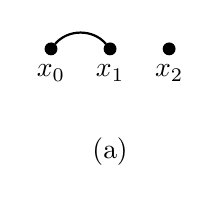
\begin{tikzpicture}[scale=1.5,font=\normalsize]
		\tikzset{
			empty node/.style={circle,inner sep=0,fill=none},
			solid node/.style={circle,draw,inner sep=1.5,fill=black},
			hollow node/.style={circle,draw,inner sep=1.5,fill=white},
			gray node/.style={circle,draw={rgb:black,1;white,4},inner sep=1.5,fill={rgb:black,1;white,4}}
		}
		\tikzset{snake it/.style={decorate, decoration=snake, line cap=round}}
		\tikzset{gray line/.style={line cap=round,thick,color={rgb:black,1;white,4}}}
		\tikzset{thick line/.style={line cap=round,rounded corners=0.1mm,thick}}
		\tikzset{thin line/.style={line cap=round,rounded corners=0.1mm}}
		\node (a)[solid node,label=below:{$x_0$}] at (-0.5,0.5) {};
		\node (b)[solid node,label=below:{$x_1$}] at (0,0.5) {};
		\node (c)[solid node,label=below:{$x_2$}] at (0.5,0.5) {};
		\node (label)[empty node,label=below:{(a)}] at (0,-0.15) {};
		\draw[thick line] (a) to[out=50,in=130] (b);
	\end{tikzpicture}
	\hspace{5mm}
	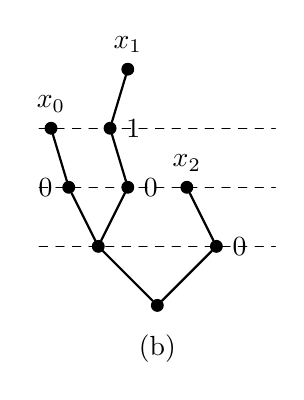
\begin{tikzpicture}[scale=1.5,font=\normalsize]
		\tikzset{
			empty node/.style={circle,inner sep=0,fill=none},
			solid node/.style={circle,draw,inner sep=1.5,fill=black},
			hollow node/.style={circle,draw,inner sep=1.5,fill=white},
			gray node/.style={circle,draw={rgb:black,1;white,4},inner sep=1.5,fill={rgb:black,1;white,4}}
		}
		\tikzset{snake it/.style={decorate, decoration=snake, line cap=round}}
		\tikzset{gray line/.style={line cap=round,thick,color={rgb:black,1;white,4}}}
		\tikzset{thick line/.style={line cap=round,rounded corners=0.1mm,thick}}
		\tikzset{thin line/.style={line cap=round,rounded corners=0.1mm}}
		\node (root)[solid node] at (0,0) {};
		\node (a)[solid node] at (-0.5,0.5) {};
		\node (b)[solid node,label=right:{$0$}] at (0.5,0.5) {};
		\node (c)[solid node,label=left:{$0$}] at (-0.75,1) {};
		\node (d)[solid node,label=right:{$0$}] at (-0.25,1) {};
		\node (e)[solid node,label=above:{$x_2$}] at (0.25,1) {};
		\node (f)[solid node,label=above:{$x_0$}] at (-0.9,1.5) {};
		\node (g)[solid node,label=right:{$1$}] at (-0.4,1.5) {};
		\node (h)[solid node,label=above:{$x_1$}] at (-0.25,2) {};
		\draw[-,thin line,dash pattern={on 3pt off 3pt}] (-1,0.5) to (1,0.5);
		\draw[-,thin line,dash pattern={on 3pt off 3pt}] (-1,1) to (1,1);
		\draw[-,thin line,dash pattern={on 3pt off 3pt}] (-1,1.5) to (1,1.5);
		\draw[thick line] (root) to (a);
		\draw[thick line] (root) to (b);
		\draw[thick line] (a) to (c);
		\draw[thick line] (a) to (d);
		\draw[thick line] (b) to (e);
		\draw[thick line] (c) to (f);
		\draw[thick line] (d) to (g);
		\draw[thick line] (g) to (h);
		\node (label)[empty node,label=below:{(b)}] at (0,-0.15) {};
	\end{tikzpicture}
	\hspace{5mm}
	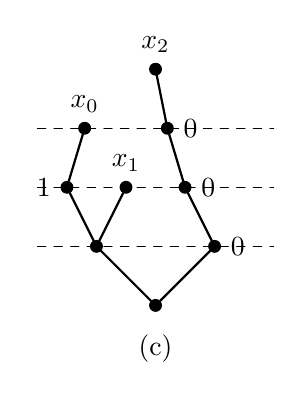
\begin{tikzpicture}[scale=1.5,font=\normalsize]
		\tikzset{
			empty node/.style={circle,inner sep=0,fill=none},
			solid node/.style={circle,draw,inner sep=1.5,fill=black},
			hollow node/.style={circle,draw,inner sep=1.5,fill=white},
			gray node/.style={circle,draw={rgb:black,1;white,4},inner sep=1.5,fill={rgb:black,1;white,4}}
		}
		\tikzset{snake it/.style={decorate, decoration=snake, line cap=round}}
		\tikzset{gray line/.style={line cap=round,thick,color={rgb:black,1;white,4}}}
		\tikzset{thick line/.style={line cap=round,rounded corners=0.1mm,thick}}
		\tikzset{thin line/.style={line cap=round,rounded corners=0.1mm}}
		\node (root)[solid node] at (0,0) {};
		\node (a)[solid node] at (-0.5,0.5) {};
		\node (b)[solid node,label=right:{$0$}] at (0.5,0.5) {};
		\node (c)[solid node,label=left:{$1$}] at (-0.75,1) {};
		\node (d)[solid node,label=above:{$x_1$}] at (-0.25,1) {};
		\node (e)[solid node,label=right:{$0$}] at (0.25,1) {};
		\node (f)[solid node,label=above:{$x_0$}] at (-0.6,1.5) {};
		\node (g)[solid node,label=right:{$0$}] at (0.1,1.5) {};
		\node (h)[solid node,label=above:{$x_2$}] at (0,2) {};
		\draw[-,thin line,dash pattern={on 3pt off 3pt}] (-1,0.5) to (1,0.5);
		\draw[-,thin line,dash pattern={on 3pt off 3pt}] (-1,1) to (1,1);
		\draw[-,thin line,dash pattern={on 3pt off 3pt}] (-1,1.5) to (1,1.5);
		\draw[thick line] (root) to (a);
		\draw[thick line] (root) to (b);
		\draw[thick line] (a) to (c);
		\draw[thick line] (a) to (d);
		\draw[thick line] (b) to (e);
		\draw[thick line] (c) to (f);
		\draw[thick line] (e) to (g) to (h);
		\node (label)[empty node,label=below:{(c)}] at (0,-0.15) {};
	\end{tikzpicture}
	\\
	\smallskip
	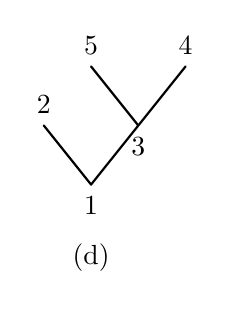
\begin{tikzpicture}[scale=1.5,font=\normalsize]
		\tikzset{
			empty node/.style={circle,inner sep=0,fill=none},
			solid node/.style={circle,draw,inner sep=1.5,fill=black},
			hollow node/.style={circle,draw,inner sep=1.5,fill=white},
			gray node/.style={circle,draw={rgb:black,1;white,4},inner sep=1.5,fill={rgb:black,1;white,4}}
		}
		\tikzset{snake it/.style={decorate, decoration=snake, line cap=round}}
		\tikzset{gray line/.style={line cap=round,thick,color={rgb:black,1;white,4}}}
		\tikzset{thick line/.style={line cap=round,rounded corners=0.1mm,thick}}
		\node (a)[empty node,label=below:{$1$}] at (0,0) {};
		\node (b)[empty node,label=above:{$2$}] at (-0.4,0.5) {};
		\node (c)[empty node,label=below:{$3$}] at (0.4,0.5) {};
		\node (d)[empty node,label=above:{$5$}] at (0,1) {};
		\node (e)[empty node,label=above:{$4$}] at (0.8,1) {};
		\draw[thick line] (a.center) to (b.center);
		\draw[thick line] (c.center) to (e.center);
		\draw[thick line] (a.center) to (c.center) to (d.center);
		\node (label)[empty node,label=below:{(d)}] at (0,-0.4) {};
	\end{tikzpicture}
	\hspace{5mm}
	\hspace{5mm}
	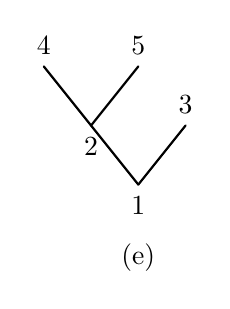
\begin{tikzpicture}[scale=1.5,font=\normalsize]
		\tikzset{
			empty node/.style={circle,inner sep=0,fill=none},
			solid node/.style={circle,draw,inner sep=1.5,fill=black},
			hollow node/.style={circle,draw,inner sep=1.5,fill=white},
			gray node/.style={circle,draw={rgb:black,1;white,4},inner sep=1.5,fill={rgb:black,1;white,4}}
		}
		\tikzset{snake it/.style={decorate, decoration=snake, line cap=round}}
		\tikzset{gray line/.style={line cap=round,thick,color={rgb:black,1;white,4}}}
		\tikzset{thick line/.style={line cap=round,rounded corners=0.1mm,thick}}
		\node (a)[empty node,label=below:{$1$}] at (0,0) {};
		\node (b)[empty node,label=below:{$2$}] at (-0.4,0.5) {};
		\node (c)[empty node,label=above:{$3$}] at (0.4,0.5) {};
		\node (d)[empty node,label=above:{$4$}] at (-0.8,1) {};
		\node (e)[empty node,label=above:{$5$}] at (0,1) {};
		\draw[thick line] (a.center) to (b.center) to (d.center);
		\draw[thick line] (b.center) to (e.center);
		\draw[thick line] (a.center) to (c.center);
		\node (label)[empty node,label=below:{(e)}] at (0,-0.4) {};
	\end{tikzpicture}
	\hspace{5mm}
	\hspace{5mm}
	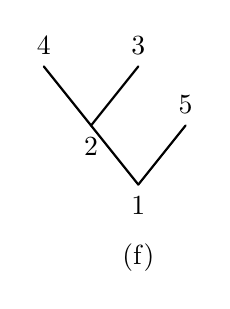
\begin{tikzpicture}[scale=1.5,font=\normalsize]
		\tikzset{
			empty node/.style={circle,inner sep=0,fill=none},
			solid node/.style={circle,draw,inner sep=1.5,fill=black},
			hollow node/.style={circle,draw,inner sep=1.5,fill=white},
			gray node/.style={circle,draw={rgb:black,1;white,4},inner sep=1.5,fill={rgb:black,1;white,4}}
		}
		\tikzset{snake it/.style={decorate, decoration=snake, line cap=round}}
		\tikzset{gray line/.style={line cap=round,thick,color={rgb:black,1;white,4}}}
		\tikzset{thick line/.style={line cap=round,rounded corners=0.1mm,thick}}
		\node (a)[empty node,label=below:{$1$}] at (0,0) {};
		\node (b)[empty node,label=below:{$2$}] at (-0.4,0.5) {};
		\node (c)[empty node,label=above:{$5$}] at (0.4,0.5) {};
		\node (d)[empty node,label=above:{$4$}] at (-0.8,1) {};
		\node (e)[empty node,label=above:{$3$}] at (0,1) {};
		\draw[thick line] (a.center) to (b.center) to (d.center);
		\draw[thick line] (b.center) to (e.center);
		\draw[thick line] (a.center) to (c.center);
		\node (label)[empty node,label=below:{(f)}] at (0,-0.4) {};
	\end{tikzpicture}
 % \includegraphics[width=10cm]{drawings/graph-representation.jpg}
\end{center}
\caption{In (a), a finite graph $G = (\{x_0, x_1, x_1\}, \{ \{x_0, x_1\}\})$. In (b) and (c), two coded Joyce graphs isomorphic to $G$. The trees (e) and (f) are Joyce trees corresponding the coded Joyce graphs (b) and (c), respectively. In (d), a Joyce tree which cannot represent the graph $G$. Indeed, since there is an edge between $x_0$ and $x_1$ but not between $x_0$ and $x_1$, then for any coded Joyce graph $\{\sigma_0, \sigma_1, \sigma_2\}$ representing $G$, $|\sigma_1 \meet \sigma_2| < |\sigma_0|$.}
\label{fig:graph-representation}
\end{figure}


\begin{theorem}[$\RCA_0$]\label{thm:joyce-graph-to-coded}
  Every countable Joyce graph is isomorphic to a coded Joyce graph.
\end{theorem}
\begin{proof}
  Let $(G, E, <, \meetlevel{\cdot}{\cdot})$ be a countable Joyce graph.
%  Let $L$ be the set of labels over $G^2$. Let $L_0=\{\meetlevel xx:x\in G\}$ and $L_1=\{\meetlevel xy:x,y\in G\land x\neq y\}$. %For every $x \in G$, let $L_x$ be the set of labels $\ell \in L$ such that $\ell <_\Nb \meetlevel{x}{x}$ and such that there is some $y \in G$ such that $y < x$ and $\meetlevel{y}{x} = \ell$.
  Let $\sigma_x \in 2^{<\omega}$ be the unique string of length $\meetlevel{x}{x}$, such that for any $j < \meetlevel{x}{x}$:
  \begin{enumerate}
  \item\label{it:jctc1} if $j=\meetlevel xy$ for some $y\in G$, then $\sigma_x(j) = 1$ if and only if $y<x$;
  \item\label{it:jctc2} if $j=\meetlevel yy$ for some $y\in G$, then $\sigma_x(j) = 1$ if and only if $xEy$;
  \item\label{it:jctc3} $\sigma_x(j)=0$ otherwise.
  \end{enumerate}
  One first need to show that $\sigma_x$ is well-defined. First, there is no $y,z\in G$ such that $\meetlevel yz = \meetlevel zz$ by \Jo3, so \Cref{it:jctc1} and \Cref{it:jctc2} are compatible. \Cref{it:jctc1} do not contradict itself as there is no $y,z\in G$ such that $\meetlevel yy=\meetlevel zz$, also by \Jo3. It remains to show that \Cref{it:jctc2} does not contradict itself: Let $x,y,z\in G$ be such that $\meetlevel xy = \meetlevel xz<\meetlevel xx$. Then, by \Jo3 $\meetlevel xy<_\Nb\meetlevel yz$ and by \Jo1 we have $x<z$ iff $x<z$. So $\sigma_x$ is well-defined.
  
Let $X = \{ \sigma_x: x \in G \}$.
We claim that $(X, \Epn, \ltlex, |\cdot \meet \cdot|)$ is a Joyce graph whose structure is isomorphic to the Joyce structure of $(G, E, <, \meetlevel{\cdot}{\cdot})$.

Let $\sigma_x, \sigma_y\in X$. We have $|\sigma_x|=\meetlevel xx\neq \meetlevel yy=|\sigma_y|$, we suppose $|\sigma_x|<|\sigma_y|$. But then, $\sigma_x\Epn\sigma_y$ iff $\sigma_y(|\sigma_x|)=1$ iff $xEy$ by \Cref{it:jctc2}.

The rest of the proof follows the same argument that the construction in the proof of \Cref{thm:joyce-orders-can-be-coded} works. 
%\pelliot{Prove the claim}
We prove that for all $x,y,z,t\in G$, $\meetlevel xy<\meetlevel zt\implies |\sigma_x\meet \sigma_y|<_\Nb|\sigma_z\meet \sigma_t|$. We actually prove the stronger fact that for every $x,y\in G$, $\meetlevel xy = |\sigma_x\meet\sigma_y|$. If $x=y$, it is clear as by construction, $\sigma_x$ is of length $\meetlevel xx$. If $x\neq y$, we first prove that $\meetlevel xy \leq |\sigma_x\meet\sigma_y|$: indeed, for all $n<\meetlevel xy$, by \Jo1, \Jo4 and the construction, we have $\sigma_x(n)=1$ iff $\sigma_y(n)=1$. It remains to show $\meetlevel xy \geq |\sigma_x\meet\sigma_y|$: if $x<y$ we have that $\sigma_x(\meetlevel xy)=0\neq 1=\sigma_y(\meetlevel xy)$ by \Cref{it:jctc1}, so $\meetlevel xy \geq |\sigma_x\meet\sigma_y|$, and similarly for $x>y$.

Let $x<y\in G$. Then, $\meetlevel xy=|\sigma_x\meet\sigma_y|$, thus $\sigma_x(|\sigma_x\meet\sigma_y|)=0\neq 1=\sigma_y(|\sigma_x\meet\sigma_y|)$ by \Cref{it:jctc2}. It follows that $\sigma_x\ltlex\sigma_y$.%as if $z$ is such that $\meetlevel xz=\meetlevel xy$, then by \Jo3 $\meetlevel xy<_\Nb\meetlevel yz$ and by \Jo1 and the fact that $x<y$, we have $x<z$. So $\sigma_x(|x\meet y|)=\sigma_x(\meetlevel xy)=0$. However, $\meetlevel xy\not\in L_y$ as witnessed by $x$, so $\sigma_y(|x\meet y|)=\sigma_y(\meetlevel xy)=1$. Therefore, $\sigma_x\ltlex\sigma_y$.

\end{proof}
\begin{corollary}
  There exists a computably coded Joyce Rado graph.
\end{corollary}
\begin{proof}
  Immediate by \Cref{thm:joyce-graph-to-coded} and \Cref{thm:joyce-rado-graph-exists}.
\end{proof}

\section{Joyce blossom graphs and an embedding theorem}

\begin{definition}\label{def:blossom-tree}\index{blossom!tree}\index{tree!blossom}\index{blossom!Joyce graph}\index{Joyce graph!blossom}
  A \emph{blossom tree} is a pair $(f, g)$
  where $f: \cantor \to \cantor$ is a $\prec$-preserving, $\ltlex$-preserving and $\meet$-preserving function, such that for every $\sigma, \tau \in \cantor$:
  \begin{enumerate}
  \item $g(\sigma) \succ f(\sigma)$; % $f(\sigma 0) \ltlex g(\sigma) \ltlex f(\sigma 1)$;
  \item if $|\tau| > |\sigma|$ then $|f(\tau)| > |g(\sigma)|$;
    % \item the function $\{\sigma, \tau\} \mapsto |g(\sigma) \meet g(\tau)|$ is injective.
  \item\label{it:blossom-rado} if $|\tau| = |\sigma|$ then
   $f(\tau 0)(|g(\sigma)|) \neq f(\tau 1)(|g(\sigma)|)$.
  \end{enumerate}
  % A \emph{blossom Joyce order} is a Joyce order of the form $(g[\cantor], \ltlex, |\cdot \meet \cdot|)$ for some blossom tree $(f, g)$.
  A \emph{Joyce blossom graph} is a structure $(g[S],\Epn,\ltlex,|\cdot\meet\cdot|)$ for some blossom tree $(f,g)$ and some set $S$ cofinal in $\cantor$ such that
   for all $\sigma,\tau\in\meetclosure S$, $|\sigma|\neq|\tau|$.
%  A \emph{Joyce blossom graph} is a Joyce blossom graph such that $(G,\Epn,\ltlex,|\cdot\meet\cdot|)$ such that there exists $(f,g)$ and $S$ such that:
\end{definition}
% \begin{definition}\label{def:blossom-tree2}
%   A \emph{blossom embedding} is a function 
%   $g: S \to \mathcal{G}$ such that  % replace f(\sigma) with g(\sigma0)\meet\sigma1
%   %is a $\prec$-preserving, $\ltlex$-preserving and $\meet$-preserving function, such that for every $\sigma, \tau \in \cantor$,
%   \begin{enumerate}
%   \item If $\sigma\meet\tau\succ \rho$ then $\meetlevel {g(\sigma)}{g(\tau)}>\meetlevel{g(\rho)}{g(\rho)}$
%   \item If $\sigma\ltlex\tau$ then $g(\sigma)<g(\tau)$
%   \item If $\sigma_0\meet\tau_0 = \sigma_0\meet\tau_0$ then $g(\sigma_0)\meet g(\tau_0) = g(\sigma_1)<g(\tau_1)$,
%   \item $g(\sigma) \succ f(\sigma)$; % $f(\sigma 0) \ltlex g(\sigma) \ltlex f(\sigma 1)$;
%   \item if $|\tau| > |\sigma|$ then $|f(\tau)| > |g(\sigma)|$.
%   \item
%     $$
%     \forall \sigma, \tau, \rho \in S \mbox{, } |\sigma|=|\rho\meet\tau|\implies \left[g(\tau)Eg(\sigma) \iff \lnot g(\rho)Eg(\sigma)\right]
%     $$

%     % \item the function $\{\sigma, \tau\} \mapsto |g(\sigma) \meet g(\tau)|$ is injective.
%   \end{enumerate}
%   % A \emph{blossom Joyce order} is a Joyce order of the form $(g[\cantor], \ltlex, |\cdot \meet \cdot|)$ for some blossom tree $(f, g)$.
%   A \emph{Joyce blossom graph} is a structure $(g[S],\Epn,\ltlex,|\cdot\meet\cdot|)$ for some $f,g:\cantor\to\cantor$ and $S\subseteq\cantor$ such that:
%   \begin{enumerate}
%     \setcounter{enumi}{3}
%   \item\label{it:blossom-cofinal} $S$ is a cofinal set with $\forall\sigma,\tau\in\meetclosure S$, $|\sigma|\neq|\tau|$;
%   \item\label{it:blossom-rado} $(f, g)$ is a blossom tree such that
%     $$
%     \forall \sigma, \rho \in 2^\ell \mbox{, } f(\rho 0)(|g(\sigma)|) \neq f(\rho 1)(|g(\sigma)|)
%     $$
%   \end{enumerate}
% %  A \emph{Joyce blossom graph} is a Joyce blossom graph such that $(G,\Epn,\ltlex,|\cdot\meet\cdot|)$ such that there exists $(f,g)$ and $S$ such that:
% \end{definition}
%\pelliot{make figures}
Note that a Joyce blossom graph $\mathcal{G}$ is a Joyce Rado graph: indeed, let $F_0$ and $F_1$ be two disjoint finite sets of vertices of $\mathcal{G}$, and let $f,g$ and $S$ be the witnesses of the fact that $\mathcal{G}$ is a Joyce blossom graph. By \Cref{it:blossom-rado} of the definition, there exists $\sigma\in f[\cantor]$ with $|\sigma|>\max\{|\tau|:\tau\in F_0\cup F_1\}$ and such that for every $\tau\in F_0\cup F_1$ $\sigma(|\tau|)=0$ iff $\tau\in F_0$. By the fact that $S$ is cofinal, let $\rho\succ f^{-1}(\sigma)$ in $S$. Then, $g(\rho)\succ \sigma$, and therefore $g(\rho)\Epn\tau$ if $\tau\in F_1$ and $\lnot g(\rho)\Epn\tau$ if $\tau\in F_0$. The Joyce requirements are satisfied by the fact that the relations are $\Epn$, $\ltlex$ and $|\cdot\meet\cdot|$, and that for all $\sigma,\tau\in\meetclosure S$, $|\sigma|\neq|\tau|$.

%Moreover, since for a blossom embedding $(f,g)$, 

%More than that, a Joyce blossom graph is a Joyce graph: By the properties of $f$ and $g$, and the fact that $\meetclosure S$ has at most one element at each level, so is for $g[S]$. The rest is ensured


Note that if $(f, g)$ is a blossom tree, then letting $B = g[\cantor]$ it follows by Item 1 that 
$(B, \preceq)$ is an antichain and $(B, \ltlex)$ contains a dense linear order with no endpoints.
From a computability-theoretic viewpoint, $\prec$-preservation of $f$ and Item 1 of  \Cref{def:blossom-tree}  ensures that if $(f, g)$ is computable, then so is $g[\cantor]$. Conversely, Item 2 of \Cref{def:blossom-tree} implies that $(f, g)$ is computable from $g[\cantor]$. One can therefore switch from one notion to the other in the computability realm.

\begin{comment}
\begin{definition}\label{def:blossom-rado-tree}
A \emph{Joyce blossom graph} is a graph $(g[S],\Epn)$ where $S$ is a cofinal set with $\forall\sigma,\tau\in\meetclosure S$, $\sigma|\neq|\tau|$ and $g$ is part of a blossom tree $(f, g)$
such that 
$$
\forall \sigma, \rho \in 2^\ell \mbox{, } f(\rho 0)(|g(\sigma)|) \neq f(\rho 1)(|g(\sigma)|)
$$
%A \emph{Joyce blossom graph} is a Joyce blossom graph of the form $(g[\cantor], \Epn, \ltlex, |\cdot \meet \cdot|)$ for some blossom Rado tree $(f, g)$.
\end{definition}
\pelliot{Make figures for these definitions}

% Note that if $(f, g)$ is a blossom Rado tree, then letting $B = g[\cantor]$, 
% $(B, \Epn)$ is a Rado graph, hence every Joyce blossom graph is a Joyce Rado graph.
%Note that if $(f, g)$ is a blossom tree, and $S\subseteq\cantor$ is a cofinal set with $\forall \sigma,\tau\in S$, $|\sigma|\neq|\tau|$, then $(g[S], \Epn)$ is a Rado graph. If $(f,g)$ is a Joyce blossom graph, then $(g[S],\Epn)$ is a Joyce Rado graph.%, hence every Joyce blossom graph is a Joyce Rado graph.

\end{comment}
\begin{lemma}\label{le:computable-bjrg}
  There exists a computable Joyce blossom graph, with a DLO induced order.
\end{lemma}
\begin{proof}
%  \pelliot{check with new definitions}
  Let $g$ and $S$ be the objects defined in the proof of \Cref{thm:joyce-rado-graph-exists}, and $\mathcal{G} =(g[S],\Epn,\ltlex,\meetlevel\cdot\cdot)$ be the Joyce graph defined in the same proof. By \Cref{thm:joyce-graph-to-coded}, let $\mathcal{G}'=(G',\Epn,\ltlex, |\cdot\meet\cdot|)$ be the coded Joyce Rado Graph computably isomorphic to $\mathcal{G}$ via $e$.%$(g[\cantor],\Epn,\ltlex,\meetlevel\cdot\cdot)$ via $e$.
%  Let $g:\cantor\to\cantor$ be the computable function defined in the proof of \Cref{thm:joyce-rado-graph-exists}. By \Cref{thm:joyce-graph-to-coded}, let $\mathcal{G}'=(G',\Epn,\ltlex, |\cdot\meet\cdot|)$ be the coded Joyce Rado Graph computably isomorphic to $(g[\cantor],\Epn,\ltlex,\meetlevel\cdot\cdot)$ via $e$.

  It remains to show that $\mathcal{G}'$ is a Joyce blossom graph. % Consider $g':\cantor\to\cantor$ to be the function such that $g(\sigma)=\tau$, where $|\tau|=3|\sigma|+2$, $\forall n<|\sigma|$, $\tau(3n)=\tau(3n+2)=\sigma(n)$ and $\tau(3n+1)=0$; and $\tau(3|\sigma|)=0$, $\tau(3|\sigma|+1)=1$. In other words, $g'$ is $\ltlex$-preserving and $\meet$-preserving and maps $\cantor$ to $G$.
  Define $g'=e\circ g$ and $f:\sigma\mapsto g'(\tau0)\meet g'(\tau1)$. It is easy to check that  $f$, $g'$ and the set $S$ are witnesses of the fact that $\mathcal{G}'$ is a Joyce blossom graph.%, via the functions. %$f,g:\cantor\to\cantor$ such that if $|\sigma|=n$, then $|f(\sigma)|=3n$, $f(\sigma)(3n)=f(\sigma)(3n+2)=\sigma(n)$ and $f(\sigma)(3n+1)=0$; and $g(\sigma)=f(\sigma)01$.
%\pelliot{Make a figure and refer to the figure.}  
\end{proof}


\begin{lemma}[$\RCA_0$]\label{thm:graph-embedding-cantor-exists}
For every Rado graph $(G, E)$,
there exists a graph embedding $e: (2^{<\omega}, \Epn) \to (G, E)$.
\end{lemma}
\begin{proof}
  Let $(\sigma_n)_{n\in\om}$ be an enumeration of $\cantor$ such that $|\sigma_n|>|\sigma_m|$ implies $n>m$. Suppose $e(\sigma_i)$ is defined for every $i<n$. Let $F_0=\{e(\tau):\tau\in\cantor, |\tau|<|\sigma_n|, \sigma_n(|\tau|)=0\}$ and $F_1=\{e(\tau):\tau\in\cantor, |\tau|<|\sigma_n|, \sigma_n(|\tau|)=1\}$. By the fact that $(G,E)$ is a Rado graph, there exists an $g\in G$ such that for all $a\in F_0$, $\lnot aEg$ and for all $a\in F_1$, $aEg$, and $g$ is not already in the image of $e$. Define $e(\sigma_n)=g$.
%\ludovic{TODO, Todorcevic}
\end{proof}

\begin{theorem}[$\ACA_0$]\label{thm:blossom-to-joyce-rado}
For every coded Joyce Rado graph $\mathcal{G}=(G,E,<,\meetlevel\cdot\cdot)$,
there is an embedding from a Joyce blossom graph to $G$.% \pelliot{why not: there is a blossom Rado subgraph?}
\end{theorem}
\begin{proof}
%  \pelliot{Adapt with new notation. One possibility is: theorem is now ``for every coded... there is an embedding from $(g[\cantor],...)$ for a blossom tree $(f,g)$''. Corollary: ``there is an embedding from a Joyce blossom graph'': same embedding works.}
We show the stronger result that there exists a blossom tree $(f,g)$ such that $(g[\cantor],\Epn,\ltlex,|\cdot\meet\cdot|)$ embeds into $\mathcal{G}$. Thus, for any $S\subseteq\cantor$ such that for all $\sigma,\tau\in \meetclosure S$ we have $|\sigma|\neq|\tau|$ whenever $\sigma\neq\tau$, we have $(g[S],\Epn,\ltlex,|\cdot\meet\cdot|)$ embeds into $\mathcal{G}$. 
  
Let $e: (\cantor, \Epn) \to (G, \Epn)$ be the graph embedding constructed in \Cref{thm:graph-embedding-cantor-exists}.
We say that $L \subseteq \cantor$ is \emph{large above $\tau \in \cantor$}
if $e^{-1}[L]$ is cofinal in $2^{<\omega}$ above $\tau$. The set $L$ is large if it is large above some $\tau \in \cantor$. Note that the collection of large sets is partition regular, that is, if $L_0 \cup \dots \cup L_{d-1}$ is large, then there is some $j < d$ such that $L_j$ is large. Moreover, if $L$ is large above $\tau$, then it is large above any $\rho \succeq \tau$. Last, $G$ is large above $\epsilon$.
Given a $\sigma \in \cantor$, we write $G \uh \sigma = \{ \tau \in G: \tau \succeq \sigma \}$.
Note that if $G \uh \sigma$ is large above $\tau$, then so is $G \uh \rho$ for every $\rho \preceq \sigma$.

The following claim is the combinatorial core of the theorem.

\begin{claim}\label{claim:blossom-to-joyce-rado-combi}
If $G \uh \sigma$ is large, then for cofinitely many $\rho \in \cantor$, there are some $\sigma_0, \sigma_1 \in G$ such that
$G \uh \sigma_0$ and $G \uh \sigma_1$ are large, $\sigma \preceq \sigma_0 \meet \sigma_1$ and $\sigma_0(\ell) \neq \sigma_1(\ell)$, where $\ell = |e(\rho)|$.
\end{claim}
\begin{proof}
Say $G \uh \sigma$ is large above some $\tau$. Pick any $\rho \in \cantor$ such that $|\rho| \geq |\tau|$. Since if $G \uh \sigma$ is large above $\tau$, $G \uh \sigma$ is large above any $\mu \succeq \tau$, then we can assume that $|\tau| = |\rho|$. Unfolding the definition of largeness,
the set $C = e^{-1}[G \uh \sigma]$ is cofinal above $\tau$. Since $e: (\cantor, \Epn) \to (G, \Epn)$ is a graph embedding and $|\tau| = |\rho|$,
then for every $\mu \succeq \tau 0$, $\neg(\mu \Epn \rho)$, hence $\neg(e(\mu) \Epn e(\rho))$ and for every $\mu \succeq \tau 1$, $\mu \Epn \rho$, hence $e(\mu) \Epn e(\rho)$. It follows that, letting $L_0 = \{\nu \in G \uh \sigma: \neg(\nu \Epn e(\rho))\}$ and $L_1 = \{\nu \in G \uh \sigma: \nu \Epn e(\rho)\}$, then  $C_0 = e^{-1}[L_0] = \{ \mu \succeq \tau 0: \mu \in C \}$ and $C_1 = e^{-1}[L_1] = \{ \mu \succeq \tau 1: \mu \in C \}$. Since $C$ is cofinal above $\tau$, then $C_0$ and $C_1$ are cofinal above $\tau 0$ and $\tau 1$, respectively, so $L_0$ and $L_1$ are large above $\tau 0$ and $\tau 1$, respectively.

Let $\ell = |e(\rho)|$. Note that since $L_0$ and $L_1$ are both non-empty, then $\ell \geq |\sigma|$.  $L_0 = \bigcup_{\nu \succeq \sigma: |\nu| = \ell} G \uh \nu 0$
and $L_1 = \bigcup_{\nu \succeq \sigma: |\nu| = \ell} G \uh \nu 1$.
By partition regularity of largeness, there are some $\nu_0, \nu_1 \succeq \sigma$
such that $|\nu_0| = |\nu_1| = \ell$, and $G \uh \nu_0 0$  and $G \uh \nu_1 1$ are large. Let $\sigma_0 = \nu_0 0$ and $\sigma_1 = \nu_1 1$. This proves our claim.
\end{proof}

We are now ready to prove \Cref{thm:blossom-to-joyce-rado}.
Using \Cref{claim:blossom-to-joyce-rado-combi}, we build a $\prec$-preserving and $\ltlex$-preserving function $\phi: \cantor \to \cantor$, together with a function $g: \cantor \to G$ such that for every $\sigma \in \cantor$:
\begin{enumerate}
	\item $G \uh \phi(\sigma)$ is large; $g(\sigma) \succeq \phi(\sigma 0) \meet \phi(\sigma 1) $;
	\item for every $\rho \in 2^{|\sigma|}$, $\phi(\rho 0)(|g(\sigma)|) \neq \phi(\rho 1)(|g(\sigma)|)$.
\end{enumerate}

Initially, $\phi(\epsilon) = \epsilon$ and $g$ is nowhere defined.
Assume $\phi$ is defined over $2^{\leq k}$ and $g$ over $2^{<k}$ for some $k \in \omega$.

\emph{Defining $\phi$}. Consider successively each $\sigma \in 2^k$. By partition regularity of largeness, $G \uh \nu$ is large for some $\nu \succeq \phi(\sigma)$ such that $|\nu|$ is bigger than any value considered so far. By \Cref{claim:blossom-to-joyce-rado-combi}, there is a $\rho$ two nodes $\mu_0, \mu_1$ extending $\nu$ such that, letting $\ell = |e(\rho)|$,  $G \uh \mu_0$ and $G \uh \mu_1$ are large and $\mu_0(\ell) < \mu_1(\ell)$.
Temporarily define $\phi(\sigma 0) = \mu_0$ and $\phi(\sigma 1) = \mu_1$. The actual value of $\phi(\sigma 0)$ and $\phi(\sigma 1)$ might change while defining $g$, but will be extensions of these strings. Since $\phi(\sigma 0) \meet \phi(\sigma 1) = \mu_0 \meet \mu_1 \succeq \nu$, $|\phi(\sigma 0) \meet \phi(\sigma 1)|$ is bigger than any value considered so far.

\emph{Defining $g$}. Consider successively each $\tau \in 2^k$. We need to define $g(\tau)$ so that it satisfies Item 2.
Since $G \uh \phi(\tau)$ is large, it is infinite, so by \Cref{claim:blossom-to-joyce-rado-combi}, there is a single $\rho$ such that $e(\rho) \succeq \phi(\tau)$ and $\ell = |e(\rho)|$ is bigger than any value considered so far, and for every $\sigma \in 2^k$ and $i < 2$ there are two extensions $\mu_0, \mu_1$ of $\phi(\sigma i)$ such that $\mu_0(\ell) < \mu_1(\ell)$. Then let $\phi(\sigma i) = \mu_i$ and $g(\tau) = e(\rho)$ and consider the next $\tau \in 2^k$.


\emph{Defining $f$}. We now define $f$ so that $(f, g)$ is a blossom tree.
For every $\sigma \in 2^{<\omega}$, let $f(\sigma) = \phi(\sigma 0) \meet \phi(\tau 0)$.
Then $f: \cantor \to \cantor$ is a $\prec$-preserving, $\ltlex$-preserving and $\meet$-preserving function such that for every $\sigma \in \cantor$:
\begin{enumerate}
	\item $g(\sigma) \succeq f(\sigma) \succeq \phi(\sigma)$;
	\item\label{it:f-g-are-rado} for every $\rho \in 2^{|\sigma|}$, $f(\rho 0)(|g(\sigma)|) \neq f(\rho 1)(|g(\sigma)|)$.
\end{enumerate}
Thus $(f, g)$ is a blossom tree, with $g:\cantor\to G$. Let $S\subseteq\cantor$ be a cofinal set such that $\meetclosure S$ has at most one string of each length. The structure $(g[S], \Epn, \ltlex, |\cdot \meet \cdot |)$ is a Joyce blossom graph. %since we ensured that the length of the elements of $g[\cantor]$ and of $f[\cantor]$ are fresh values, so are unique. Thus  $(g[\cantor], \Epn, \ltlex, |\cdot \meet \cdot |)$ is a Joyce blossom graph. Moreover, it is a substructure of $G$. This completes the proof of \Cref{thm:blossom-to-joyce-rado}.
\end{proof}

\begin{theorem}[$\RCA_0$]\label{thm:joyce-to-rado-blossom}
For every Joyce blossom graph $\mathcal{G}$
and every (finite or infinite) Joyce graph $\mathcal{F}$,
there is a Joyce structure embedding from $\mathcal{F}$ to $\mathcal{G}$.
\end{theorem}
\begin{proof}
Let $(f, g)$ be the blossom tree and $S\subseteq\cantor$ such that $\mathcal{G} = (g[S], \Epn, \ltlex, |\cdot \meet \cdot|)$.
  Let $F\subseteq\cantor$ be the domain of a coded Joyce graph isomorphic to $\mathcal{F}$. Let $D=\{d_i:i\in|\meetclosure F|\}$ be an enumeration of $\meetclosure F$ such that $i<j$ implies $|d_i|<|d_j|$. We first build a function $\phi:D\to S$. Define $\phi(d_0)$ to be any element of $S$. Suppose $\phi(d_i)$ is defined for $i<n$. Then $d_n$ is mapped to any element of $S$ extending $\sigma$, where $\sigma$ is the string of length $|\phi(n-1)|+1$, such that:
  \begin{enumerate}
  \item\label{it:jtrb0} if $k<|\sigma|$ and $k\neq|\phi(d_i)|$ for any $i<n$, then $\sigma(k)=0$;
  \item\label{it:jtrb1} if $d_i\prec d_n$, then $\sigma(|\phi(d_i)|)=1$ iff $d_i1\prec d_n$;
  % \item\label{it:jtrb2} Otherwise $\sigma(|\phi(d_i)|)=j$ so that $f((\sigma\uh |\phi(d_i)|)\cat j)(|g(\phi(d_i))|)=d_n(|d_i|)$.
  \item\label{it:jtrb2} Otherwise $\sigma(|\phi(d_i)|)=j$ so that $f(\sigma)(|g(\phi(d_i))|)=d_n(|d_i|)$.
  \end{enumerate}
  The last item can be satisfy for a single $j$ by \Cref{it:blossom-rado} of \Cref{def:blossom-tree}. The string $\sigma$ is uniquely defined, and $\phi(d_n)\in S$ extending $\sigma$ exists as $S$ is cofinal. Note that $\phi$ is $\prec$-preserving: if $d_n\prec d_m$, then by \Cref{it:jtrb0}, for any $k<|\phi(d_n)|$ if $k\not\in\{|\phi(d_i):i<n\}$, then $\phi(d_n)(k)=\phi(d_m)(k)$. By \Cref{it:jtrb1} for any $i$ such that $d_i\prec d_n$, $\phi(d_n)(|\phi(d_i)|)=\phi(d_m)(|\phi(d_i)|)$. By \Cref{it:jtrb2} and the fact that $f$ is $\prec$-preserving, for $i$ such that $d_i\not\prec d_n$, we again have $\phi(d_n)(|\phi(d_i)|)=\phi(d_m)(|\phi(d_i)|)$. So $\phi$ is $\prec$-preserving.

  Define $\psi = g\circ\phi$. We claim that $\psi:F\to g[S]$ preserves the Joyce graph structure. In order to show the claim, we have to prove that it preserves $\ltlex$, and that for any $d_{n_0},d_{n_1},d_{m_0},d_{m_1}\in F$, $|d_{n_0}\meet d_{n_1}|<|d_{m_0}\meet d_{m_1}|$ implies $|\psi(d_{n_0})\meet \psi(d_{n_1})|<|\psi(d_{m_0})\meet \psi(d_{m_1})|$, and finally that for any $d_n,d_m\in F$, $d_n\Epn d_m$ implies $\psi(d_n)\Epn \psi(d_m)$. The proof of these three facts are respectively in the three following paragraphs.
  
  The fact that $\phi$ is $\prec$-preserving implies that $\phi(d_n\meet d_m)\prec\phi(d_n)\meet\phi(d_m)$. By \Cref{it:jtrb1}, $\phi(d_n\meet d_m)\succ\phi(d_n)\meet\phi(d_m)$: indeed, $\phi(d_n)(|\phi(d_n\meet d_m)|)\neq \phi(d_m)(\phi(|d_n\meet d_m|))$. So $\phi$ is $\meet$-preserving, and by \Cref{it:jtrb1}, it is also $\ltlex$-preserving. The function $g$ is also $\ltlex$-preserving: $f$ is $\ltlex$-preserving, and $f(\sigma)\prec g(\sigma)$ for every $\sigma\in\cantor$. So $\psi=g\circ\phi$ is $\ltlex$-preserving.

  % By construction, $|d_n|<|d_m|\iff n<m\iff |\phi(d_n)|<|\phi(d_m)|$. 
  By the second item of \Cref{def:blossom-tree}, for all $\sigma,\tau\in\cantor$ with $|\sigma|\neq|\tau|$, $|\sigma|<|\tau|\iff |g(\sigma)|<|g(\tau)|\iff |f(\sigma)|<|f(\tau)|\iff |g(\sigma)|<|f(\tau)|\iff |f(\sigma)|<|g(\tau)|$. So $|d_n|<|d_m|\iff |\psi(d_n)|<|\psi(d_m)|$. Now, suppose $|d_{n_0}\meet d_{n_1}|<|d_{m_0}\meet d_{m_1}|$ for some $d_{n_0},d_{n_1},d_{m_0}d_{m_1}\in F$. Let $d_n=d_{n_0}\meet d_{n_1}$ and $d_m=d_{m_0}\meet d_{m_1}$. If $d_{n_0}\neq d_{n_1}$, then $\psi(d_{n_0})\meet\psi(d_{n_1})=f(\phi(d_n))$, otherwise $\psi(d_{n_0})\meet\psi(d_{n_1})=g(\phi(d_n))$; and similarly for $m_0, m_1, m$ with $d_m=d_{m_0}\meet d_{m_1}$. So, depending whether $d_n, d_m\in F$, we use one of the previous equivalence to get that  $|\psi(d_{n_0})\meet \psi(d_{n_1})|<|\psi(d_{m_0})\meet \psi(d_{m_1})|$.
  
%   Indeed, as $g$ preserves $\ltlex$ and the ordering of the meets: that is, by the second item of \Cref{def:blossom-tree}, $\forall\sigma,\tau\in\cantor$ with $|\sigma|\neq|\tau|$, $|\sigma|<|\tau|\iff |g(\sigma)|<|g(\tau)|$. Since these properties are also satisfied by $\phi$, they are satisfied by $\psi$.

  Finally, for any $n<m$,
  \[
  	\psi(d_m)(|\psi(d_n)|)= g(\phi(d_m))(|g(\phi(d_n))|)=f(\phi(d_m))(|g(\phi(d_n))|)
  \]
  as $g(\phi(d_m))\succ f(\phi(d_m))$. By \Cref{it:jtrb2} $\phi(d_m)$ is chosen so that $f(\phi(d_m))(|\psi(d_n)|)= d_m(|d_n|)$.
  % First, note that by construction, $\phi$ is $\prec$-preserving. Combined with the first item, we have that $\phi$ is $\meet$-preserving. By Item 1 again, it is also $\ltlex$-preserving.
\end{proof}

\begin{corollary}[$\ACA_0$]\label{th:4.1LaflammeRado}
  Let $\mathcal{G}$ be a Joyce Rado graph, and $\mathcal{F}$ be a (finite or infinite) Joyce graph. Then, there exists an embedding from $\mathcal{F}$ to $\mathcal{G}$.
\end{corollary}
\begin{proof}
By \Cref{thm:joyce-graph-to-coded}, we can assume that $\mathcal{G}$ is a coded Joyce Rado graph.
By \Cref{thm:blossom-to-joyce-rado}, there is an embedding of a Joyce blossom graph $\mathcal{B}$ to $\mathcal{G}$. By \Cref{thm:joyce-to-rado-blossom},
there is an embedding of $\mathcal{F}$ to $\mathcal{B}$. Thus there is an embedding of $\mathcal{F}$ to $\mathcal{G}$.
\end{proof}

Recall that the \emph{age} of a graph $\mathcal{G}$ is the collection of all finite graphs that are isomorphic to a subgraph of $\mathcal{G}$.

\begin{corollary}
  The age of a Joyce Rado graph is the set of finite Joyce graphs.
\end{corollary}

%\begin{lemma}[$\ACA_0$]
%For every coded Joyce Rado graph $G$,
%for every graph embedding $e: (2^{<\omega}, \Epn) \to G$,
%there exist two $\prec$-preserving injective functions $f, g: 2^{<\omega} \to 2^{<\omega}$
%such that $f[2^{<\omega}] \subseteq G^{\meet} \setminus G$
%and for every $\sigma \in 2^{<\omega}$, letting $U_\sigma = \{\tau \in G: \tau \succeq f(\sigma) \}$,
%$e^{-1}[U_\sigma]$ is cofinal in $2^{<\omega}$ above $g(\sigma)$.
%\end{lemma}
%\begin{proof}
%We say that $L \subseteq \cantor$ is \emph{large above $\tau \in \cantor$}
%if $e^{-1}[L]$ is cofinal in $2^{<\omega}$ above $\tau$. The set $L$ is large if it is large above some $\tau \in \cantor$. Note that the collection of large sets is partition regular, that is, if $L_0 \cup \dots \cup L_{d-1}$ is large, then there is some $j < d$ such that $L_j$ is large. Moreover, if $L$ is large above $\tau$, then it is large above any $\rho \succeq \tau$. Last, $G$ is large above $\epsilon$.
%
%Given a $\sigma \in \cantor$, we write $G \uh \sigma = \{ \tau \in G: \tau \succeq \sigma \}$.
%Reformulating the statement of the lemma, there exists $f$ and $g$ such that $f[2^{<\omega}] \subseteq G^{\meet} \setminus G$ and for every $\sigma \in \cantor$, $G \uh f(\sigma)$ is large above $g(\sigma)$.
%
%
%A tree $T \subseteq 2^{<\omega}$ is \emph{2-branching} if for non-leaf $\sigma \in T$, both $\sigma0$ and $\sigma1$ belong to $T$. For every $k$, define a finite 2-branching tree $T_k \subseteq \cantor$, and two $\prec$-preserving functions $g_k, \phi_k: T_k \to \cantor$, so that:
%\begin{enumerate}
%	\item $T_k \subset T_{k+1}$, $g_k \subset g_{k+1}$, $\phi_k \subset \phi_{k+1}$; $\bigcup_k T_k = 2^{<\omega}$;
%	\item For every $\sigma \in \leaves(T_k)$, $G \uh \phi_k(\sigma)$ is large above $g_k(\sigma)$.
%\end{enumerate}
%Then define $g = \bigcup_k g_k$, $\phi = \bigcup_k \phi_k$, and for every $\sigma \in 2^{<\omega}$, $f(\sigma) = \phi(\sigma0) \meet \phi(\tau0)$. First, note that $G \uh \phi(\sigma 0)$ is large above $g(\sigma 0)$ and $G \uh \phi(\sigma 1)$ is large above $g(\sigma 1)$, so there exists some $\tau_0 \in G \uh \phi(\sigma 0)$ and $\tau_1 \in G \uh \phi(\sigma 1)$ such that $f(\sigma) = \tau_0 \meet \tau_1$, so by definition of $G^{\meet}$, $f(\sigma) \in G^{\meet}$. Moreover, by Item 2
%
%First, $T_0 = \{\epsilon\}$, $f_0$ is nowhere defined, $g_0(\epsilon) = \epsilon$
%and $\phi_0(\epsilon) = \epsilon$. Note that Item 2 is vacuously satisfied, and Item 3 holds since $G \uh \phi_0(\epsilon) = G$, which is large above $g_0(\epsilon) = \epsilon$. 
%
%Assume $T_k, g_k, f_k$ and $\phi_k$ are defined.
%Fix a leaf $\sigma \in T_k$. 
%By Item 3, $G \uh \phi_k(\sigma)$ is large above $g_k(\sigma)$.
%Let $\ell = |\phi_k(\sigma)|$. We claim that 
%
%%Then, by partition regularity 
%%First, $g(\epsilon) = \epsilon$ and $f(\epsilon) = e(0) \meet e(1)$. Note that 
%%$e^{-1}[G \uh e(\epsilon)] = e^{-1}[G] = 2^{<\omega}$, which is cofinal in $\cantor$ above $\epsilon = g(\epsilon)$, so $G \uh 
%%
%%We build a sequence of finite 2-branching trees $T_0 \subseteq T_1 \subseteq \dots$
%%such that $\bigcup_n T_n = 2^{<\omega}$, together with a pair sequence of partial functions $f_0, f_1, \dots$ and $
%
%
%\ludovic{TODO}
%\end{proof}

\begin{theorem}
There is a computable Joyce Rado graph $\mathcal{G}$ such that for every Joyce blossom graph $\mathcal{B}$,
every embedding of $\mathcal{B}$ to $\mathcal{G}$ computes $\emptyset'$.
\end{theorem}
\begin{proof}
  % We will build a computable Joyce Rado graph $(G,\Epn, \ltlex, \meetlevel\cdot\cdot)$ where $G\subseteq\cantor$, such that the following hold:
  % \begin{itemize}
  % \item[$\Rc$:] For every $\sigma,\tau\in G$, there exists infinitely many $\rho, \gamma$ such that $\sigma\meet\tau=\rho\meet\gamma$ if and only if $\emptyset'\uh|\sigma\meet\gamma|=\emptyset'_{|\sigma|}\uh|\sigma\meet\gamma|$
  % \end{itemize}
  % Suppose that such a $G$ is defined. Then, for any $f,g$ Joyce blossom graph with $g[\cantor]\subseteq G$, $g$ compute $\emptyset'$: For any $n$, there exists $\sigma,\tau\in\cantor$ such that $|g(\sigma)\meet g(\tau)|>n$, and as $f(\sigma\meet\tau) = g(\sigma)\meet g(\tau)$, for any $\rho,\gamma$ such that $\rho\meet\gamma=\sigma\meet\tau$, $g(\sigma)\meet g(\tau) = g(\rho)\meet g(\gamma)$ and as there are infinitely many such $\rho,\gamma$, by the requirement, $\emptyset'\uh|\sigma\meet\gamma|=\emptyset'_{|\sigma|}\uh|\sigma\meet\gamma|$.
%  Note that if  $|\sigma\meet\tau|<|\rho\meet\gamma|$ implies $\meetlevel\sigma\tau<\meetlevel\rho\gamma$, if $\mathcal{B}$ is a Joyce blossom graph and $e:\mathcal{B}\to(G,\Epn,\ltlex,\meetlevel\cdot\cdot)$ is an embedding, then $e\circ f:\cantor\to\meetclosure G$, $e\circ g:\cantor\to G$ form a blossom graph.
  
  The idea of the proof is to build a Joyce Rado graph with domain $G$ such that if $S\subseteq\cantor$ is a cofinal set with at most one meet of each length, $f:\cantor\to \meetclosure G$ and $g:\cantor\to G$ form a blossom tree, and $\sigma,\tau\in\cantor$ are such that $|g(\sigma)\meet g(\tau)|>3j$, then $\emptyset'(j)=1$ iff $g(\sigma)(3j+2)=g(\sigma)(3j+2)$ iff $g(\tau)(3j+2)=g(\tau)(3j+2)$. 
  
  % Here is the construction. 
  Let $(G_0,E)$ be a Rado graph, and let $(g_n)_{n\in\om}$ be an enumeration of $G_0$, and $(\emptyset'_s)_{s\in\om}$ a computable approximation of $\emptyset'$. Define $\sigma_n$ to be the unique string of length $3n+2$ such that:
  \begin{enumerate}
  \item $\sigma_n(3n)=0$ and $\sigma_n(3n+1)=1$;
  \item for any $j<n$, $\sigma_n(3j+1)=0$ and
    \begin{enumerate}
    \item if $\emptyset'_n(j)=0$ and $g_nEg_j$ then $\sigma_n(3j)=0$ and $\sigma_n(3j+2)=1$,
    \item if $\emptyset'_n(j)=0$ and $\lnot g_nEg_j$ then $\sigma_n(3j)=1$ and $\sigma_n(3j+2)=0$ ,
    \item if $\emptyset'_n(j)=1$ and $g_nEg_j$ then $\sigma_n(3j)=1$ and $\sigma_n(3j+2)=1$,
    \item if $\emptyset'_n(j)=1$ and $\lnot g_nEg_j$ then $\sigma_n(3j)=0$ and $\sigma_n(3j+2)=0$.
    \end{enumerate}
  \end{enumerate}
  Let $G = \{\sigma_n:n\in\Nb\}$. It is clear that $(G,\Epn)$ is a Rado graph, as it is in bijection with $G_0$ via $g_n\mapsto \sigma_n$ since $g_nEg_m$ iff $\sigma_n\Epn\sigma_m$. Define $\meetlevel{\sigma_n}{\sigma_m}=v(\sigma_n\meet\sigma_m)$ where $v$ is a fixed injective function $\cantor\to\om$ such that if $|\sigma|<|\tau|$ then $v(\sigma)<v(\tau)$. Then by construction, $\mathcal{G}=(G,\Epn,\ltlex,\meetlevel\cdot\cdot)$ is a Joyce Rado graph.

  Now, suppose that $f:\cantor\to \meetclosure G$ and $g:\cantor\to G$ form a Joyce blossom graph.
  The claim is the following: if $\sigma,\tau\in\cantor$ are such that $|g(\sigma)\meet g(\tau)|>3j$, then $\emptyset'(j)=1$ iff $g(\sigma)(3j+2)=g(\sigma)(3j+2)$ iff $g(\tau)(3j+2)=g(\tau)(3j+2)$.

  Indeed, recall that $g(\sigma)\meet g(\tau)=f(\sigma)\meet f(\tau)$. Let $\rho\succ\sigma$ be such that $|g(\rho)|\geq 3n+2$ where $\emptyset'_{n}(j)=\emptyset'(j)$. By construction, $g(\rho)(3j)=g(\rho)(3j+2)$ iff $\emptyset'_{n}(j)=1$ iff $\emptyset'(j)=1$. As $\rho\succ\sigma$, we have $g(\rho)\succ f(\sigma)\prec g(\sigma)$ so finally $g(\sigma)(3j)=g(\sigma)(3j+2)$ iff $\emptyset'(j)=1$. % As $g(\sigma)\succ f(\sigma)$, $g(\sigma)(3j)=g(\sigma)(3j+2)$ iff $\emptyset'(j)=1$.

  Therefore, given $g$, to know the value of $\emptyset'(j)$, it suffices to find $\sigma,\tau\in S$ such that $|g(\sigma)\meet g(\tau)|>3j$, and answer according to whether $g(\sigma)(3j)=g(\sigma)(3j+2)$.
\end{proof}

\begin{corollary}
\Cref{th:4.1LaflammeRado} implies $\ACA_0$.
\end{corollary}

\section{A proof of the Rado Graph theorem}\label{subsect:rado-from-mtt}


\begin{definition}\index{diagonalization!Joyce graph}\index{Joyce graph!diagonalization}
A \emph{Joyce graph diagonalization} for some Joyce graph $(U, E_U,  <_U, \meetlevel{\cdot}{\cdot}_U)$ is a function $h: 2^{<\omega} \to U$, such that for every coded Joyce graph $X$,
$(h[X], E_U, <_U, \meetlevel{\cdot}{\cdot}_U)$ is isomorphic to $X$.
\end{definition}

\begin{theorem}[$\RCA_0$]\label{thm:joyce-diagonalization-Rado}
There exists a Joyce Rado graph $(2^{<\omega}, E_T, <_T, \meetlevel{\cdot}{\cdot}_T)$
such that for every coded Joyce order $X$,
the Joyce structures of $(X, E_T, <_T, \meetlevel{\cdot}{\cdot}_T)$ and $(X, \Epn, \ltlex, |\cdot \meet \cdot|)$ are isomorphic.
\end{theorem}
\begin{proof}
Let $(U, \Epn, \ltlex, \meetlevel{\cdot}{\cdot}_U)$ be the Joyce Rado graph defined in \Cref{thm:joyce-rado-graph-exists}, that is, $U = (000 \cup 101)^{*}01$ and $\meetlevel{\sigma}{\tau}_U = v(\sigma \meet \tau)$ for some injective function $v: 2^{<\omega} \to \omega$ such that 
for every $\sigma, \tau \in 2^{<\omega}$, if $|\sigma| < |\tau|$ then $v(\sigma) < v(\tau)$.

Define the Joyce Rado graph $(2^{<\omega}, \Epn, <_T,  \meetlevel{\cdot}{\cdot}_T)$ as follows:
Given $\sigma \in 2^{<\omega}$, let $\hat{\sigma}$ be the binary string of length $3|\sigma|+2$
defined for every $j < |\sigma|$ by $\hat{\sigma}(3j) = \sigma(j)$, $\hat{\sigma}(3j+1) = \hat{\sigma}(3j+2) = 0$, and $\hat{\sigma}(3|\sigma|) = 0$ and $\hat{\sigma}(3|\sigma|+1) = 1$.
For instance, if $\sigma = 0110$ then $\hat{\sigma} = 00010010000001$.
Then let $\sigma <_T \tau$ if and only if $\hat{\sigma} \ltlex \hat{\tau}$
and $\meetlevel{\sigma}{\tau}_T = \meetlevel{\hat{\sigma}}{\hat{\tau}}_U$. 

Let $X$ be a coded Joyce order. We claim that $(X, \Epn, <_T, \meetlevel{\cdot}{\cdot}_T)$ and $(X, \Epn, \ltlex, |\cdot \meet \cdot|)$ are isomorphic.

Fix $\sigma, \tau \in X$. If $\sigma \ltlex \tau$, then $\hat{\sigma} \ltlex \hat{\tau}$, hence $\sigma <_T \tau$. Conversely, if $\sigma <_T \tau$, then $\hat{\sigma} \ltlex \hat{\tau}$, but since $\sigma$ and $\tau$ are incomparable with respect to the prefix relation, this implies that $\sigma \ltlex \tau$. Thus $\sigma <_T \tau$ if and only if $\sigma \ltlex \tau$.

Fix $\sigma, \tau, \rho, \mu \in X$. If $|\sigma \meet \tau| <_\Nb |\rho \meet \mu|$, then 
$|\hat{\sigma} \meet \hat{\tau}| <_\Nb |\hat{\rho} \meet \hat{\mu}|$, then $v(\hat{\sigma} \meet \hat{\tau}) <_\Nb v(\hat{\rho} \meet \hat{\mu})$, hence $\meetlevel{\sigma}{\tau}_T <_\Nb \meetlevel{\rho}{\mu}_T$. Conversely, assume $\meetlevel{\sigma}{\tau}_T <_\Nb \meetlevel{\rho}{\mu}_T$. Unfolding the definition, $v(\hat{\sigma} \meet \hat{\tau}) <_\Nb v(\hat{\rho} \meet \hat{\mu})$. If $|\hat{\sigma} \meet \hat{\tau}| \neq |\hat{\rho} \meet \hat{\mu}|$, then by definition of $v$, $|\hat{\sigma} \meet \hat{\tau}| <_\Nb |\hat{\rho} \meet \hat{\mu}|$, hence $|\sigma \meet \tau| <_\Nb |\rho \meet \mu|$. If $|\hat{\sigma} \meet \hat{\tau}| = |\hat{\rho} \meet \hat{\mu}|$, then since $X$ is a coded Joyce graph, $\sigma \meet \tau = \rho \meet \mu$, so $\hat{\sigma} \meet \hat{\tau} = \hat{\rho} \meet \hat{\mu}$ and $v(\hat{\sigma} \meet \hat{\tau}) = v(\hat{\rho} \meet \hat{\mu})$, contradiction. 
\end{proof}

\begin{corollary}[$\ACA_0$]\label{cor:joyce-diagonalization-exists-Rado}
  Every Joyce Rado graph $(U, E_U, <_U, \meetlevel\cdot\cdot_U)$ has a Joyce graph diagonalization.
\end{corollary}
\begin{proof}
Let $(2^{<\omega}, E_T, <_T, \meetlevel{\cdot}{\cdot}_T)$ be the Joyce Rado graph of \Cref{thm:joyce-diagonalization-Rado}. By \Cref{th:4.1LaflammeRado}, there is an embedding $h: 2^{<\omega} \to U$. By definition of an embedding, for every coded Joyce graph $X \subseteq 2^{<\omega}$, $(h[X], E_U, <_U, \meetlevel{\cdot}{\cdot}_U)$ is isomorphic to $(X, E_T, <_T, \meetlevel{\cdot}{\cdot}_T)$. By \Cref{thm:joyce-diagonalization-Rado}, $(X, E_T, <_T, \meetlevel{\cdot}{\cdot}_T)$ is isomorphic to $(X, \Epn, \ltlex, |\cdot \meet \cdot|)$. Thus $h$ is a Joyce graph diagonalization.
\end{proof}

In the case of Joyce blossom graphs, the existence of a Joyce graph diagonalization holds in $\RCA_0$;

\begin{corollary}[$\RCA_0$]\label{cor:joyce-diagonalization-exists-blossom}
  Every Joyce blossom graph has a Joyce graph diagonalization.
\end{corollary}
\begin{proof}
Similar to the proof of \Cref{cor:joyce-diagonalization-exists-Rado},
but apply \Cref{thm:joyce-to-rado-blossom} instead of \Cref{th:4.1LaflammeRado}.
\end{proof}

\begin{lemma}\label{lem:coded-joyce-order-to-strong-subtree-Rado}
Let $F$ be a finite coded Joyce graph of size $n$ and $T \in \Subtree{\omega}{2^{<\omega}}$.
Then every $E \in \Subtree{2n-1}{T}$ contains at most one coded Joyce graph isomorphic to $F$. Moreover, every coded Joyce graph $H \subseteq T$ isomorphic to $F$
	is included in some $E \in \Subtree{2n-1}{T}$.
\end{lemma}
\begin{proof}
The proof is a straightforward adaptation of \Cref{lem:coded-joyce-order-to-strong-subtree}, \emph{mutatis mutandis}.
\end{proof}

\begin{theorem}[$\ACA_0$]\label{thm:strong-rado-one-type}
  Let $\mathcal{G}$ be a Joyce Rado structure, and $\mathcal{F}$ be a finite Joyce graph. Then, the big Ramsey number of $\mathcal{F}$ in $\mathcal{G}$ is 1.
\end{theorem}
\begin{proof}
Let $X$ be a countable coded Joyce Rado graph and $F$ be a finite coded Joyce Rado graph of size $n$. Fix a coloring $f: {X \choose F} \to k$. Here, ${X \choose F}$ denotes all the subcopies of $F$ in $X$.

Let $h: 2^{<\omega} \to X$ be a Joyce graph diagonalization, which exists by \Cref{cor:joyce-diagonalization-exists-Rado}. Let $g: \Subtree{n}{2^{<\omega}} \to k$ be defined for every $E \in \Subtree{2n-1}{2^{<\omega}}$ by $g(E) = f(h(H))$ where $H \subseteq E$ is the unique element coded Joyce graph isomorphic to $F$, if it exists. Otherwise let $g(E) = 0$. This coloring is well-defined by \Cref{lem:coded-joyce-order-to-strong-subtree}.


By Milliken's tree theorem for height $2n-1$, there is a strong subtree $S \in \Subtree{\omega}{2^{<\omega}}$ such that $g$ restricted to $\Subtree{2n-1}{S}$ is monochromatic for some color $i < k$. In particular, by \Cref{lem:coded-joyce-order-to-strong-subtree-Rado}, for every coded Joyce graph $H \subseteq S$ isomorphic to $F$, there is some $E \in \Subtree{2n-1}{S}$ containing $H$, and $g(E) = f(h(H)) = i$.

Since $S \in \Subtree{\omega}{2^{<\omega}}$, there is an injective function $\phi: 2^{<\omega} \to S$ such that $\phi[X]$ is a coded Joyce graph isomorphic to $X$. In particular, since $h$ is a Joyce graph diagonalization, $Y = h[\phi[X]]$ is a coded Joyce Rado graph isomorphic to $X$, hence a subcopy of~$X$.

We claim that $f$ restricted to ${Y \choose F}$ is monochromatic for color~$i$.
Let $\hat{H}$ be a copy of $F$ in $Y = h[\phi[X]]$. Let $H \subseteq \phi[X]$ be such that $h[H] = \hat{H}$. In particular since $\phi[X]$ is a coded Joyce graph, so is $H$, so since $h$ is a Joyce graph diagonalization, $\hat{H} = h[H]$ is a coded Joyce graph isomorphic to $H$. In other words, $H$ is a copy of $F$ in $\phi[X] \subseteq S$, so $H$ is a copy of $F$ in $S$. By choice of $S$, $f(h[H]) = i$, so $f(\hat{H}) = i$. This completes the proof of \Cref{thm:strong-rado-one-type}.
\end{proof}

\begin{corollary}[$\ACA_0$]
  The statement $(\forall k) \JRG^n_{k,J_n}$ holds, where $J_n$ is the number of non isomorphic Joyce graph structure with $n$ elements, while $(\forall k)\JRG^n_{k,J_n-1}$ does not hold.
\end{corollary}
\begin{proof}
Let $\ell$ be the number of Joyce graph with $n$ elements. Let $F_0, \dots, F_{\ell-1}$ be a finite enumeration of all the finite coded Joyce graph structures of size $n$.

We first prove that $\JRG^n_{k, \ell}$ holds.
Fix a coloring $f: [X]^n \to k$ for some countable Joyce Rado graph structure $(X, E, <, \JRel)$. By \Cref{thm:strong-devlin-one-type}, build a finite decreasing sequence of subsets $X = X_0 \supseteq X_1 \supseteq \dots \subseteq X_\ell$ of $X$ such that for every $s < \ell$:
\begin{enumerate}
	\item $(X_{s+1},  E, <, \JRel)$ is a subcopy of $(X_s, E, <, \JRel)$;
	\item every copy of $F$ in $(X_{s+1},  E, <, \JRel)$ is monochromatic for $f$ for some color $i_s < k$
\end{enumerate}
The Joyce graph structure $(X_\ell, E, <, \JRel)$ is a subcopy of $(X, <, \JRel)$.
Moreover, for every $E \in [X_\ell]^n$, $(E, <, \JRel)$ is isomorphic to $F_s$ for some $s < k$,
so $f(E) = i_s$. It follows that $f[X_\ell]^n \subseteq \{ i_s: s < \ell \}$, hence $|f[X_\ell]^n| \leq \ell$.

We now show that the bound is tight. Let $f: [X]^n \to k$ be defined by $f(H) = s$ for the unique $s < \ell$ such that $(H, E, <, \JRel)$ is isomorphic to $F_s$. 
Let $(Y, E, <, \JRel)$ be a subcopy of $(X, E, <, \JRel)$. In particular, $(Y, E, <, \JRel)$ is a Joyce Rado graph structure, so by \Cref{th:4.1LaflammeRado}, for every $s < \ell$, there is an embedding of $F_s$ into $(Y, E, <, \JRel)$. Therefore, $|f[Y]^n| \geq \ell$.
\end{proof}


\begin{theorem}[$\ACA_0$]\label{thm:subgraph-to-subjoyce-Rado}
  Let $\mathcal{G}=(G,E,<,\JRel)$ be a Joyce graph structure. Let $\mathcal{G}'=(g',E)$ be an isomorphic subcopy of $(G,E)$, that is, a Rado graph. Then, there exists a subcopy $(G'',E)$ of $(G',E)$ such that $(G'',E,<,\JRel)$ is a subcopy of $\mathcal{G}$.
\end{theorem}
\begin{proof}
  The structure $\hat\Xb'=(X',E, <,\JRel)$ is a Joyce Rado graph structure, even if it might not be isomorphic to $\Xb$. By \Cref{th:4.1LaflammeRado}, there exists an embedding of $\Xb$ into $\hat\Xb'$. The image of the embedding is $\Xb''$.
\end{proof}

Note that contrary to the case of Joyce orders, for which the proof that Devlin's theorem implies the Joyce Devlin theorem holds in $\RCA_0$, the following corollary holds in $\ACA_0$. The difference comes from proof of \Cref{th:4.1LaflammeRado} which is more complex than \Cref{th:4.1LaflammeDevlin}.

\begin{corollary}[$\ACA_0$]
  The Rado Graph theorem for $n$-tuples and $\ell$ colors implies the Joyce Rado graph theorem for $n$-tuples and $\ell$ colors.
\end{corollary}

\begin{corollary}[$\ACA_0$]
  The tight bound for the Rado graph theorem and the Joyce Rado graph theorem for $n$ elements are the same, that is, the number of Joyce graph structures with $n$ elements.
\end{corollary}
\begin{proof}
Let $b_0$ and $b_1$ be the tight bound for the Rado graph theorem and the Joyce Rado graph theorem for $n$ elements, respectively. 

We first claim that $b_0 \leq b_1$. 
Let $(X, E)$ be a Rado graph. By \Cref{cor:rado-can-be-enriched}, one can enrich this graph with an order $<$ and a relation $\JRel$ so that $(X, E, <, \JRel)$ is a Joyce Rado graph structure. Let $f: [X]^n \to k$ be a coloring. By choice of $b_1$, there is a Joyce subcopy $(Y, E, <, \JRel)$ of $(X, E, <, \JRel)$ such that $|f[Y]^n| \leq b_1$. In particular, $(Y, E)$ is a subcopy of $(X, E)$ so $b_0 \leq b_1$.

We then claim that $b_1 \leq b_0$.
Let $(X, E, <, \JRel)$ be a Joyce Rado graph structure.  Let $f: [X]^n \to k$ be a coloring. By choice of $b_0$, there is a subcopy $(Y, E)$ of $(X, E)$ such that $|f[Y]^n| \leq b_0$. 
By \Cref{thm:subgraph-to-subjoyce-Rado}, there is a subcopy $(Z, E)$ of $(Y, E)$ such that $(Z, E, <, \JRel)$ is a Joyce subcopy of $(X, E, <, \JRel)$. In particular, $|f[Z]^n| \leq b_0$. Thus $b_1 \leq b_0$.

It follows that $b_0 = b_1$. Moreover, by \Cref{cor:strong-devlin-tight-joyce-orders}, this tight bound is the number of Joyce graph structures with $n$ elements.
\end{proof}
  

\section{Cone avoidance of the Rado Graph theorem for pairs}

\begin{theorem}\label{thm:blossom-limit-cone-avoidance}
Fix two sets $C$ and $Z$ such that $C \not \leq_T Z$.
Let
\[
	\mathcal{B} = (B, \Epn, \ltlex, |\cdot \meet \cdot|)
\]
be a $Z$-computable Joyce blossom graph. For every $Z$-computable function $f: [B]^2 \to k$, there exists a subcopy $(U, \Epn, \ltlex, |\cdot \meet \cdot|)$ of $\mathcal{B}$ and a finite set of colors $I \subseteq k$ such that $C \not \leq_T U \oplus Z$, $|I| \leq 4$, and 
$$
(\forall \ell_0)( \forall^{\infty} \ell_1)( \forall^{\infty} \ell_2)[ f[U(\ell_0, \ell_1, \ell_2)]^2 \subseteq I],
$$
where $U(\ell_0, \ell_1, \ell_2)$ is the set of Joyce subgraphs of size 2 whose labels are exactly $\ell_0, \ell_1, \ell_2$, that is,  $U(\ell_0, \ell_1, \ell_2) = \{ \{\sigma, \tau\} \in [U]^2: |\sigma \meet \tau| = \ell_0, |\sigma| = \ell_1, |\tau| = \ell_2 \}$.
\end{theorem}
\begin{proof}
By \Cref{cor:joyce-diagonalization-exists-blossom}, there is a $Z$-computable Joyce graph diagonalization $h: \cantor \to B$.
Let $\mathcal{F}_0, \mathcal{F}_1, \mathcal{F}_2, \mathcal{F}_3$ be the 4 Joyce graph structures of size 2.

For every $j < k$, let $g_j: \Subtree{3}{2^{<\omega}} \to k$ be defined for every $E \in \Subtree{3}{2^{<\omega}}$ by $g(E) = f(h(H))$ where $H \subseteq E$ is the unique element coded Joyce graph isomorphic to $\mathcal{F}_j$, if it exists. Otherwise let $g(E) = 0$. This coloring is well-defined by \Cref{lem:coded-joyce-order-to-strong-subtree}.


By 4 successive applications of \Cref{thm:cmtt-admits-strong-cone-avoidance}, there exists a strong subtree $R \in \Subtree{\omega}{2^{<\omega}}$ such that for each $j < 4$, $g_j$ restricted to $\Subtree{3}{R}$ is stable. For each $j < 4$, let $\hat{g}_j: \Subtree{2}{R} \to k$
 be the (non-computable) limit coloring of $g_j$. 
 
 Again, by 4 successive applications of \Cref{thm:cmtt-admits-strong-cone-avoidance}, there exists a strong subtree $S \in \Subtree{\omega}{R}$ such that for each $j < 4$, $\hat{g}_j$ restricted to $\Subtree{2}{S}$ is stable. For each $j < 4$, let $\mu_j: S \to k$
 be the (non-computable) limit coloring of $\hat{g}_j$.
 
 Last, by 4 successive applications of \Cref{thm:hl-strong-cone-avoidance},
 there exists a strong subtree $T \in \Subtree{\omega}{T}$ such that for each $j < 4$,
 $\mu_j$ restricted to $T$ is monochromatic for some color $i_j < 4$. Let $I = \{i_j: j < 4\}$.


In particular, by \Cref{lem:coded-joyce-order-to-strong-subtree-Rado}, for every coded Joyce graph $H \subseteq T$ isomorphic to $\mathcal{F}_j$, there is some $E \in \Subtree{3}{S}$ containing $H$, and $g_j(E) = f(h(H))$.

Let $(X, \Epn, \ltlex, |\cdot \meet \cdot|)$ be a $Z$-computable coded Joyce graph isomorphic to $\mathcal{B}$, which exists by \Cref{thm:joyce-graph-to-coded}.
Since $T \in \Subtree{\omega}{2^{<\omega}}$, there is an injective function $\phi: 2^{<\omega} \to T$ such that $\phi[X]$ is a coded Joyce graph isomorphic to $X$, hence to $\mathcal{B}$. In particular, since $h$ is a Joyce graph diagonalization, $U = h[\phi[X]]$ is a coded Joyce Rado graph isomorphic to $X$, hence a subcopy of~$\mathcal{B}$.

We claim that the statement of the theorem holds for $U$, $f$ and $I$.
Given any $\ell \in \omega$, there is at most one level $n \in \omega$ such that for every $\sigma, \tau \in T$ with $|\sigma \meet \tau| = n$, $|h(\phi(\sigma)) \meet h(\phi(\tau))| = \ell$. We call $n$ the \emph{preimage} of $\ell$. Moreover, if $\ell$ is a label of $U$, that is, there is some $\rho, \nu \in U$ such that $|\rho \meet \nu| = \ell$, then it has a preimage. 

Fix $\ell_0 \in \omega$. If $\ell_0$ has no preimage, then $U(\ell_0, \ell_1, \ell_2) = \emptyset$ for every $\ell_1, \ell_2$ and the property is vacuously satisfied. Let $n_0$ be the preimage of $\ell_0$. Since for every $j < 4$, $\hat{g}_j$ is stable over $\Subtree{\omega}{T}$ with limit color $i_j$, there is some threshold $t_0 \in \omega$ such that for every strong subtree $E$ of $U$ of height 2 whose first level is $n_0$ and second is higher than $t_0$, $\hat{g}_j(E) = i_j$. For all but finitely many $\ell_1$, the preimage of $\ell_1$, if it exists, is larger than $t_0$. Fix any such $\ell_1$ with preimage $n_1$. For every $j < 4$, since $\hat{g}_j$ is the limit coloring of $g_j$, there is a threshold $t_1 \in \omega$ such that for every strong subtree $E$ of height 3 whose first two levels are $n_0$ and $n_1$, respectively, and whose last level is higher than $t_1$, $g_j(E) = i_j$. 
	For all but finitely many $\ell_2$, its preimage is larger than $t_1$. 
	
	Fix any such $\ell_2$, and let $\hat{H} \in U(\ell_0, \ell_1, \ell_2)$. 
	Let $j < 4$ be such that $\hat{H}$ is isomorphic to $\mathcal{F}_j$. Let $H \subseteq \phi[X]$ be such that $h[H] = \hat{H}$. In particular since $\phi[X]$ is a coded Joyce graph, so is $H$, so since $h$ is a Joyce graph diagonalization, $\hat{H} = h[H]$ is a coded Joyce graph isomorphic to $H$. In other words, $H$ is a copy of $\hat{H}$ in $\phi[X] \subseteq T$, so $H$ is a copy of $\mathcal{F}_j$ in $T$. By choice of $T$, $f(h[H]) = i_j$, so $f(\hat{H}) = i_j \in I$.
This completes the proof of \Cref{thm:blossom-limit-cone-avoidance}.
\end{proof}

\begin{theorem}\label{thm:weak-rado-cone-avoidance}
$(\forall k)\RG^2_{k, 4}$ admits cone avoidance.
\end{theorem}
\begin{proof}
Fix two sets $Z, C$ such that $C \not \leq_T Z$.
Let $(V, E)$ be a $Z$-computable Rado graph and $h: [V]^2 \to k$ be a $Z$-computable coloring.

By computable categoricity of the Rado graph, $(V, E)$ is $Z$-computably isomorphic to the graph of a computable Joyce blossom graph $\mathcal{B} = (B, \Epn, \ltlex, |\cdot \meet \cdot|)$.
This induces a $Z$-computable coloring $\hat{h}: [B]^2 \to k$ by composing the coloring $h$ with the isomorphism.
By \Cref{thm:blossom-limit-cone-avoidance}, there is a subcopy $(U, \Epn, \ltlex, |\cdot \meet \cdot|)$ of $\mathcal{B}$ and a finite set of colors $I \subseteq k$ such that $C \not \leq_T U \oplus Z$, $|I| \leq 4$, and 
\begin{equation}\label{eqn:weak-rado-pairs-ca-1}
(\forall \ell_0)( \forall^{\infty} \ell_1)( \forall^{\infty} \ell_2)[ \hat{h}[U(\ell_0, \ell_1, \ell_2)]^2 \subseteq I],
\end{equation}
where $U(\ell_0, \ell_1, \ell_2)$ is the set of Joyce subgraphs of size 2 whose labels are exactly $\ell_0, \ell_1, \ell_2$, that is, $U(\ell_0, \ell_1, \ell_2) = \{ \{\sigma, \tau\} \in [U]^2: |\sigma \meet \tau| = \ell_0, |\sigma| = \ell_1, |\tau| = \ell_2 \}$.
Let $(f, g)$ be a $U \oplus Z$-computable blossom tree and $D \subseteq \cantor$ be a $Z$-computable set cofinal in $\cantor$ such that $g[D] = B$. 
In particular, by \Cref{eqn:weak-rado-pairs-ca-1}, the following holds:
\begin{equation}\label{eqn:weak-rado-pairs-ca-2}
(\forall \rho \in \cantor)(\forall^{\infty} \sigma_0 \in D)(\forall^{\infty} \sigma_1 \in D)[\sigma_0 \meet \sigma_1 = \rho \Rightarrow \hat{h}(g(\sigma_0), g(\sigma_1)) \in I].
\end{equation}

We are going to build a by forcing infinite set $G \subseteq D$ such that $(g[G], \Epn)$ is a Rado graph and $\hat{h}[g[G]]^2 \subseteq I$. 

\begin{definition}
A string $\sigma \in \cantor$ \emph{witnesses} a finite 2-partition $F_0 \sqcup F_1 \subseteq \cantor$
if for every $i < 2$ and every $\rho \in F_i$, $\sigma(|\rho|) = i$.
\end{definition}

In other words, $\sigma$ witnesses $F_0 \sqcup F_1 \subseteq \cantor$ if in the graph $(\cantor, \Epn)$, $\sigma$ is connected to all the elements of $F_1$ and disconnected from all the elements of $F_0$.
Note that if $\sigma$ witnesses  $F_0 \sqcup F_1 \subseteq D$, then so does any $\tau \succeq \sigma$.

\begin{lemma}\label{lem:weak-rado-cone-avoidance-Rado-preservation}
If $(G, \Epn)$ is a Rado graph for some $G \subseteq D$, then so is $(g[G], \Epn)$.	
\end{lemma}
\begin{proof}
Let $\hat{F}_0 \sqcup \hat{F}_1 \subseteq g[G]$ be a finite 2-partition. 
Let $F_0 = g^{-1}[\hat{F}_0]$ and $F_1 = g^{-1}[\hat{F}_1]$. In particular, $F_0$ and $F_1$ are disjoint. 
Since $(G, \Epn)$ is a Rado graph, then there is some $\sigma \in G$ witnessing the 2-partition $F_0 \sqcup F_1 \subseteq G$. We claim that $g(\sigma)$ witnesses the 2-partition $\hat{F}_0 \sqcup \hat{F}_1 \subseteq g[G]$. By definition of a blossom tree $(f,g)$, the function $f$ is $\meet$-preserving, so $f(\sigma)$ witnesses the 2-partition $\hat{F}_0 \sqcup \hat{F}_1 \subseteq g[G]$. Since $g(\sigma) \succeq f(\sigma)$, then so does $g(\sigma)$.
\end{proof}


Given $\sigma \in \cantor$, we write $D \uh \cantor = \{ \tau \in D: \tau \succeq \sigma \}$.
Given a finite set $R \subseteq \cantor$, we write $D \uh R = \{ \tau \in D: (\exists \sigma \in R)[\tau \succeq \sigma] \}$.

\begin{definition}
A \emph{condition} is a pair $(F, R)$ where $F \subseteq D$ and $R \subseteq \cantor$
are both finite sets such that $R$ is prefix-free and:
\begin{enumerate}[(1)]
	\item every finite 2-partition $F_0 \sqcup F_1 = F$ is witnessed by some $\sigma \in R$;
	\item for every $\sigma \in F$ and $\tau \in F \cup (D \uh R)$, $\hat{h}(g(\sigma), g(\tau)) \in I$;
%	\item For every $\sigma_0 \neq \sigma_1 \in R$ and $\tau_0 \in D \uh \sigma_0$ and $\tau_1 \in D \uh \sigma_1$, $\hat{h}(g(\tau_0), g(\tau_1)) \in I$.
\end{enumerate}
A condition $(E, S)$ \emph{extends} $(F, R)$ (written $(E, S) \leq (F, R)$) if $F \subseteq E$, $E \setminus F \subseteq D \uh R$ and for every $\tau \in S$, there is some $\sigma \in R$ such that $\tau \succeq \sigma$.
\end{definition}

One can see a condition $(F, R)$ as the Mathias condition $(F, D \uh R)$.
In particular, for every filter $\Fc$ for this notion of forcing, letting $G_\Fc = \bigcup \{ F: (F, R) \in \Fc \}$, if $(F, R) \in \Fc$ then $F \subseteq G_\Fc \subseteq F \cup (D \uh R)$.
Structurally, we ensured that $\hat{h}[g[G_\Fc]]^2 \subseteq I$. Note that $(\emptyset, \{\epsilon\})$ is a valid condition.

\begin{lemma}\label{lem:weak-rado-cone-avoidance-condition-is-rado}
For every condition $(F, R)$, $(F \cup (D \uh R), \Epn)$ is a Rado graph.	
\end{lemma}
\begin{proof}
Fix any finite 2-partition  $E_0 \sqcup E_1 \subseteq F \cup D \uh R$.
By definition of a condition, there is some $\sigma \in R$ witnessing the 2-partition $E_0 \cap F, E_1 \cap F$. Since $D$ is cofinal in $\cantor$, there is some $\tau \in D$ such that $\tau \succeq \sigma$, and for every $i < 2$ and $\rho \in E_i \setminus F$, $\tau(|\rho|) = i$. 
Thus $\tau$ witnesses the 2-partition $E_0 \sqcup E_1 \subseteq F \cup D \uh R$. Moreover $\tau \in D \uh \sigma$, hence $\tau \in D \uh R$.
\end{proof}

The following lemma shows that if $\Fc$ is a sufficiently generic filter, then $(G_\Fc, \Epn)$ is a Rado graph.

\begin{lemma}\label{lem:weak-rado-cone-avoidance-progress}
For every condition $(F, R)$ and every 2-partition $F_0 \sqcup F_1 \subseteq F$,
an extension $(E, S)$ such that $E$ contains an element witnessing the 2-partition.
\end{lemma}
\begin{proof}
Let $\ell_0 \in \omega$ be larger than the length of any string in $R$.
Let $\ell_1 \in \omega$ be sufficiently large with respect to $\ell$ so that
\begin{equation}\label{eqn:weak-rado-pairs-ca-3}
(\forall \rho \in 2^{\leq \ell_0})(\forall \sigma_0 \in D^{\geq \ell_1})(\forall^{\infty} \sigma_1 \in D)[\sigma_0 \meet \sigma_1 = \rho \Rightarrow \hat{h}(g(\sigma_0), g(\sigma_1)) \in I].
\end{equation}
Such an $\ell_1$ exists by \Cref{eqn:weak-rado-pairs-ca-2}.
Let $\hat{R}$ be obtained from $R$ by extending each string $\sigma \in R$ into a string $\tau$ of length $\ell_1$ such that $\tau(\ell_0) = 0$.
Then $(F, \hat{R})$ is again a condition.

By \Cref{lem:weak-rado-cone-avoidance-condition-is-rado}, since $(F \cup (D \uh \hat{R}), \Epn)$ is a Rado graph, there is some $\tau \in F \cup (D \uh \hat{R})$ witnessing the 2-partition.
If $\tau \in F$ then we are done since $(F, \hat{R})$ then satisfies the lemma, so assume $\tau \in D \uh \hat{R}$. % By cofinality of $D$ in $\cantor$, we can assume that $|\tau|$ is bigger than the maximal length of the strings in $R$. 
Let $E = F \cup \{\tau\}$. Since $|\tau| \geq \ell_1$, by \Cref{eqn:weak-rado-pairs-ca-3}, there is some $\ell_2 \in \omega$ so that
\begin{equation}\label{eqn:weak-rado-pairs-ca-4}
(\forall \rho \in 2^{\leq \ell_0})(\forall \mu \in D^{\geq \ell_2})[\tau \meet \mu = \rho \Rightarrow \hat{h}(g(\tau), g(\mu)) \in I].
\end{equation}
For every $\sigma \in R$, let $\sigma_0, \sigma_1 \in R$ be strings of length at least $\ell_2$ such that $\sigma_0(|\tau|) = 0$, $\sigma_1(|\tau|) = 1$, $\sigma_0(\ell_0) = \sigma_1(\ell_0) = 1$, $\sigma_0 \meet \sigma_1 \succeq \sigma$, and define $S = \{\sigma_0, \sigma_1: \sigma \in R \}$.

We claim that $(E, S)$ is a condition.
We first prove Item (1). Let $F_0 \sqcup F_1 \subseteq E$ be a 2-partition. Since $(F, R)$ is a condition, there is some $\sigma \in R$ witnessing the 2-partition $(F_0 \setminus \{\tau\}) \sqcup  (F_1 \setminus \{\tau\})$. If $\tau \in F_i$ for some $i < 2$, then $\sigma_i \succeq \sigma$ witnesses the 2-partition  $F_0 \sqcup F_1 \subseteq E$. If $\tau \not \in F_0 \sqcup F_1$, then any $\sigma_i \succeq \sigma$ witnesses it.

We now prove Item (2). Fix $\nu \in E$ and $\mu \in E \cup (D \uh S)$ with $|\nu| \leq |\mu|$. If $\nu \neq \tau$, then $\nu \in F$ and $\hat{h}(g(\nu), g(\mu)) \in I$ by Item (2) for $(F, R)$.
If $\nu = \tau$, then $\mu \in (D \uh S)$. By choice of $S$, $\mu(\ell_0) = 1$, and $\nu(\ell_1) = 0$. Thus, $|\mu \meet \nu| \leq \ell_0$. Moreover, since every string in $S$ has length at least $\ell_2$, $|\mu| \geq \ell_2$, so by \Cref{eqn:weak-rado-pairs-ca-4}, $\hat{h}(g(\nu), g(\mu)) \in I$.
\end{proof}

\begin{definition}
Let $c = (F, R)$ be a condition and let $\varphi(G, x)$ be a $\Delta^{0,Z}_0$ formula with a free set parameter $G$ and a free integer parameter $x$.
\begin{enumerate}[1.]
	\item $c \Vdash (\exists x)\varphi(G, x)$ if $\varphi(F, x)$ holds for some $x \in \omega$;
	\item $c \Vdash (\forall x)\varphi(G, x)$ if $\varphi(F \cup E, x)$ holds for every $x \in \omega$ and every $E \subseteq D \uh R$ such that $\hat{h}[g[E]]^2 \subseteq I$.
\end{enumerate}
\end{definition}

In particular, the forcing relation is closed under extension, and if $\Fc$ is a filter and $c \Vdash \varphi(G)$ for some $\Sigma^{0,Z}_1$ or $\Pi^{0,Z}_1$ formula and some $c \in \Fc$, then $\varphi(G_\Fc)$ actually holds. As usual, we write $c \Vdash \Gamma^{G \oplus Z} \neq C$ if either $c \Vdash \Gamma^{G \oplus Z}(x)\uparrow$ or $c \Vdash \Gamma^{G \oplus Z}(x)\downarrow \neq C(x)$ for some $x \in \omega$.

\begin{lemma}\label{lem:weak-rado-cone-avoidance-req}
For every condition $c$ and every Turing functional $\Gamma$,
there is an extension $d$ of $c$ such that $d \Vdash \Gamma^{G \oplus Z} \neq C$.
\end{lemma}
\begin{proof}
As in the proof of \Cref{lem:weak-rado-cone-avoidance-progress}, let $\ell_0$ and $\ell_1$ be sufficiently large to satisfy \Cref{eqn:weak-rado-pairs-ca-3}. Again, let $\hat{R}$ be obtained from $R$ by extending each string $\sigma \in R$ into a string $\tau$ of length $\ell_1$ such that $\tau(\ell_0) = 0$.

Let $W$ be the set of all pairs $(x, v) \in \omega \times 2$ such that there is a finite set $E \subseteq D \uh \hat{R}$ satisfying $\hat{h}[g[E]]^2 \subseteq I$ and such that $\Phi^{(F \cup E) \oplus Z}(x) \downarrow = v$. Note that the set $W$ is $Z$-c.e. We have three cases.

\case{1}{$(x, 1-C(x)) \in W$ for some $x \in \omega$.} Let $E \subseteq D \uh \hat{R}$ witness that $(x, 1-C(x)) \in W$, that is, $\hat{h}[g[E]]^2 \subseteq I$ and $\Phi^{(F \cup E) \oplus Z}(x) \downarrow = 1-C(x)$. Since for every $\tau \in E$, $|\tau| \geq \ell_1$, then by \Cref{eqn:weak-rado-pairs-ca-3}, there is some $\ell_2 \in \omega$ so that
\begin{equation}\label{eqn:weak-rado-pairs-ca-5}
(\forall \rho \in 2^{\leq \ell_0})(\forall \tau \in E)(\forall \mu \in D^{\geq \ell_2})[\tau \meet \mu = \rho \Rightarrow \hat{h}(g(\tau), g(\mu)) \in I].
\end{equation}

For every $\sigma \in R$, and every 2-partition $E_0 \sqcup E_1 = E$, let $\sigma_{E_0, E_1}$ be a string of length at least $\ell_2$ extending $\sigma$, such that $\sigma_{E_0, E_1}(|\tau|) = 0$ for every $\tau \in E_0$ and $\sigma_{E_0, E_1}(|\tau|) = 1$ for every $\tau \in E_1$. Let $S = \{\sigma_{E_0, E_1}: \sigma \in R, E_0 \sqcup E_1 = E \}$.

We claim that $(F \cup E, S)$ is a condition.
We first prove Item (1). Let $(F_0 \cup E_0) \sqcup (F_1 \cup E_1) \subseteq F \cup E$ be a 2-partition with $F_0 \sqcup F_1 \subseteq F$ and $E_0 \sqcup E_1 \subseteq E$. Since $(F, R)$ is a condition, there is some $\sigma \in R$ witnessing the 2-partition $F_0 \sqcup F_1 \subseteq F$. By construction, $\sigma_{E_0, E_1} \in S$ witnesses the 2-partition $E_0 \sqcup E_1 \subseteq E$ and extends $\sigma$, so $\sigma_{E_0, E_1}$ witnesses the 2-partition $(F_0 \cup E_0) \sqcup (F_1 \cup E_1) \subseteq F \cup E$.

We now prove Item (2). Fix $\nu \in F \cup E$ and $\mu \in F \cup E \cup (D \uh S)$ with $|\nu| \leq |\mu|$. If $\nu \in F$, then $\hat{h}(g(\nu), g(\mu)) \in I$ by Item (2) for $(F, R)$.
If $\nu \in E$ and $\mu \in F \cup E$, then $\mu \in E$ since $|\nu| \leq |\mu|$, and $\hat{h}(g(\nu), g(\mu)) \in I$ since $\hat{h}[g[E]]^2 \subseteq I$.
If $\nu \in \tau$ and $\mu \in (D \uh S)$, then by choice of $S$, $\mu(\ell_0) = 1$, and $\nu(\ell_1) = 0$. Thus, $|\mu \meet \nu| \leq \ell_0$. Moreover, since every string in $S$ has length at least $\ell_2$, $|\mu| \geq \ell_2$, so by \Cref{eqn:weak-rado-pairs-ca-5}, $\hat{h}(g(\nu), g(\mu)) \in I$.

Moreover, the condition $(F \cup E, S)$ forces $\Phi^{G \oplus Z}(x)\downarrow = 1-C(x)$, thus satisfies the lemma.

\case{2}{$(x, C(x)) \not \in W$ for some $x \in \omega$.} Then the condition $(F, \hat{R})$ is an extension of $(F, R)$ forcing $\Phi^{G \oplus Z}(x)\uparrow \vee \Phi^{G \oplus Z}(x)\downarrow \neq C(x)$, and we are done.

\case{3}{otherwise.} Then $W$ is a $Z$-c.e.\ graph of the characteristic function of $C$, hence $C$ is $Z$-computable, contradicting the hypothesis. This case therefore cannot happen. This completes the proof of \Cref{lem:weak-rado-cone-avoidance-req}.
\end{proof}


We are now ready to prove \Cref{thm:weak-rado-cone-avoidance}.
Let $\Fc$ be a sufficiently generic filter for this notion of forcing.
By definition of a forcing condition, $\hat{h}[g[F]]^2 \subseteq I$ for every $(F, R) \in \Fc$, so $\hat{h}[g[G_\Fc]]^2 \subseteq I$. By \Cref{lem:weak-rado-cone-avoidance-req}, $C \not \leq_T G_\Fc \oplus Z$. Since $g \leq_T Z$ then $C \not \leq_T g[G_\Fc] \oplus Z$. By \Cref{lem:weak-rado-cone-avoidance-progress}, $(G_\Fc, \Epn)$ is a Rado graph, and by \Cref{lem:weak-rado-cone-avoidance-Rado-preservation}, so is $(g[G_\Fc], \Epn)$. 
The image of $(g[G_\Fc], \Epn)$ be the $Z$-computable isomorphism between the Rado graph $(V, E)$ and the Joyce blossom graph $\mathcal{B}$ yields a Rado subgraph $(\hat{V}, E)$ of $(V, E)$ such that $h[\hat{V}]^2 \subseteq I$ and $C \not \leq_T \hat{V} \oplus Z$.
This completes the proof of \Cref{thm:weak-rado-cone-avoidance}.
\end{proof}

\begin{corollary}
$(\forall k)\RG^2_{k, 4}$ does not imply $\ACA_0$ over $\RCA_0$.
\end{corollary}
\begin{proof}
Immediate by \Cref{thm:weak-rado-cone-avoidance} and \Cref{lem:cone-avoidance-not-aca}.
\end{proof}

\section{Lower bound on the Rado Graph theorem}
In order to show lower bounds, we  use the notion of Joyce blossom graph: Indeed, one can computably embed any Joyce graph in a Joyce blossom graph by \Cref{thm:joyce-to-rado-blossom}, and there is a computable one by \Cref{le:computable-bjrg}.  %we embed are a dense linear order, or a linear order, into a computable Joyce blossom graph.
The embeddings of a Joyce complete graph with order type $\Nb$ or $\Qb$ allow to show that $\JRG^2_{8,7}$ implies respectively $\RT22$ and the Devlin Theorem. Even though it is weaker, We include the proof of $\RT22$ from $\JRG^2_{8,7}$ as it yields a computable reduction.
% \begin{corollary}
%   For any Joyce graph $\mathcal{F}$ with two elements, the statement $\JRG^F_{<\infty}$ implies $\RT22$.
% \end{corollary}
\begin{theorem}
  For every $k,n$, the statement $\JRG^2_{4k, 4n+3}$ implies $\RT2{k,n}$. In particular, $\JRG^2_{8, 7}$ implies $\RT22$.
\end{theorem}
\begin{proof}
  We first give the insight about what $4n+3$ corresponds to: if the union of $4$ disjoints sets is of cardinality $4n+3$, then one of them is of cardinality at most $N$.
  \begin{claim}\label{cl:Joyce-complete-linear-graph}
    There exists a Joyce graph $(G,E,<,\meetlevel\cdot\cdot)$ such that $(G,E)$ is the complete graph and for all $a,b\in G$, $a<b\iff \meetlevel aa<\meetlevel bb$.
  \end{claim}
  \begin{proof}
    Let $G=\{1^{2n}0:n\geq 1\}$, then $(G,\Epn, \ltlex, |\cdot\meet\cdot|)$ is a witness of the claim.    
  \end{proof}
Let $f:\Nb^2\to k$ be a symmetric coloring. By \Cref{le:computable-bjrg}, let $\mathcal{G}=(G,E,<,\meetlevel\cdot\cdot)$ be a computable Joyce blossom graph. %In particular, there exists an embedding $e$ from $(G,\ltlex)$ to $\Xb$.

  Let $(\mathcal{F}_i)_{i<4}$ be an enumeration of the finite Joyce graph structures with two elements. If $a,b\in G$, define $g(a,b)=\langle f(\meetlevel aa, \meetlevel bb), i\rangle$ where $i$ is such that $\{a,b\}$ is isomorphic to $\mathcal{F}_i$. By $\JRG^2_{<\infty, 2n+1}$, let $\mathcal{G}'$ be a subcopy of $\mathcal{G}$ in $\mathcal{G}$, using at most $4n+3$ colors. Either $\{(a,b):aEb\}$ or $\{(a,b):\lnot aEb\}$ uses at most $2n+1$ colors, suppose for instance that it is the former. Similarly, either $\{(a,b):a<b\land \meetlevel aa<\meetlevel bb\land aEb\}$ or $\{(a,b):a<b\land \meetlevel aa>\meetlevel bb\land aEb\}$ uses at most $n$ colors, suppose that it is the former. By \Cref{cl:Joyce-complete-linear-graph} there exists a Joyce complete graph $\Kb$ such that  for all $a,b\in \Kb$, $a<b\iff \meetlevel aa<\meetlevel bb$. By \Cref{thm:joyce-to-rado-blossom}, there exists a computable subcopy $\mathcal{G}''$ of $\Kb$ inside $\mathcal{G}'$. In particular, $\mathcal{G}''$ uses at most $n$ colors for $g$. As a consequence, $\{\meetlevel aa:a\in\mathcal{G}''\}$ uses at most $n$ colors for $f$.
  % Thus, $\JRG^2_{8, 7}$ implies $\DT2{4,3}$ which implies $\ACA_0$.
  % Let $f:\Nb\to2$ be a coloring. By \Cref{th:exists-dense-rado-graph}, let $E,<,\meetlevel\cdot\cdot$ be such that $(\Nb,E,<,\meetlevel\cdot\cdot)$ is a densely Rado graph. Let $(s_i)_{i<4}$ be an enumeration of the Joyce graph structure with $2$ elements, and define $g:[\Nb]^2\to 8$ such that $g(n,m)=(f(n,m), i)$ where $(\{n,m\},E,<,\meetlevel\cdot\cdot)$ is isomorphic to $s_i$.
  % By $\JRG^2_{<\infty, 7}$, let $S\subseteq\Nb$ such that $|g[\Nb^2]|\leq7$. As $7<2\times 4$, let $i$ be such that $\{(n,m):n,m\in S$ and $\{n;m\}$ is isomorphic to $s_i\}$ is monochromatic for $g$, and thus also for $f$. The rest of the proof is the same as the previous corollary for $F=s_i$.
\end{proof}

\begin{theorem}
  For every $n,k$, the statement $\JRG^2_{2k, 2n+1}$ implies $\DT2{k,n}$ and thus $\JRG^2_{8, 7}$ implies $\ACA_0$.
\end{theorem}
\begin{proof}
  We start with a claim.
  \begin{claim}\label{cl:Joyce-complete-dlo-graph}
    There exists a Joyce graph $(G,E,<,\meetlevel\cdot\cdot)$ such that $(G,E)$ is the complete graph and $(G,<)$ is a DLO.
  \end{claim}
  \begin{proof}
    Let $(G,<,\meetlevel\cdot\cdot)$ be a DLO Joyce order. Define $E=\{(a,b):a,b\in G\}$. Then $(G, E,<,\meetlevel\cdot\cdot)$ is a witness of the claim.
  \end{proof}
  Let $\Xb=(X,<_X)$ be a computable dense linear order with no endpoints, and $f:X^2\to k$ be a symmetric coloring. By \Cref{le:computable-bjrg}, let $\mathcal{G}$ be a computable Joyce blossom graph. In particular, there exists an embedding $e$ from $(G,\ltlex)$ to $\Xb$.

  If $a,b\in G$, define $g(a,b)=\langle f(e[\{a;b\}]), 1\rangle$ if $aEb$ and
  \[
  g(a,b)=\langle f(e[\{a;b\}]), 0\rangle
  \]
  if $\lnot aEb$. By $\JRG^2_{<\infty, 2n+1}$, let $\mathcal{G}'$ be a subcopy of $\mathcal{G}$ in $\mathcal{G}$, using at most $2n+1$ colors. Either $\{(a,b):aEb\}$ or $\{(a,b):\lnot aEb\}$ uses at most $n$ colors, suppose for instance that it is the former. By \Cref{cl:Joyce-complete-dlo-graph} there exists a Joyce complete graph $\Kb$ whose order is a DLO. By \Cref{thm:joyce-to-rado-blossom}, there exists a computable subcopy $\mathcal{G}''$ of $\Kb$ inside $\mathcal{G}'$. In particular, $\mathcal{G}''$ is a DLO and uses at most $n$ colors for $g$. As a consequence, $e[\mathcal{G}'']\subseteq\Xb$ is a DLO and uses at most $n$ colors for $f$.

  Thus, $\JRG^2_{8, 7}$ implies $\DT2{4,3}$ which implies $\ACA_0$.
\end{proof}


% \begin{theorem}
%   Let $\mathcal{G}=(G,E,<,\meetlevel\cdot\cdot)$ be a DLO Joyce Rado graph. Then, there exists $G'\subseteq G$ such that $(G',E)$ is the completely disconnected countable graph, and $(G', <)$ is a dense linear order.
% \end{theorem}
% \begin{corollary}
%   The Joyce Rado Theorem implies Devlin's theorem, and therefore $\ACA_0$.
% \end{corollary}

Larson~\cite{MR2488745} computed the big Ramsey number for small subgraphs of the Rado graph.
The sum of the big Ramsey numbers for subgraphs of size 3 is equal to the number of Joyce graphs of size 3, that is, 112. In other words, $(\forall k)\RG^3_{k, 112}$ holds, while $(\forall k)\RG^3_{k, 111}$ does not. In the particular case of the complete graph $K_3$ of size 3,
$(\forall k)\RG^{K_3}_{k, 16}$ holds, while $(\forall k)\RG^{K_3}_{k, 15}$ does not.

%\begin{theorem}[{Hirschfeldt and Jockusch~\cite[Theorem 2.1]{Hirschfeldt2016notions}}]\label{thm:unbalanced-rt32-pazp}
%There exists a computable coloring $h: [\omega]^3 \to 2$, such that every infinite $h$-homogeneous set is of PA degree over $\emptyset'$. Moreover, there is a function $\mu: \omega \to \omega$ such that for every $x, y, z$ such that $\mu(x) < y$ and $\mu(y) < z$, then $h(\{x, y, z\}) = 1$.
%\end{theorem}

The proof technique for the following theorem stems from Jockusch~\cite{Jockusch1972Ramseys} who constructed a computable instance of Ramsey's theorem for triples whose solutions compute the halting set. It was later refined by Hirschfeldt and Jockusch~\cite[Theorem 2.1]{Hirschfeldt2016notions} who showed the existence of a computable such instance such that every solution is of PA degrees over $\emptyset'$. Although it is unknown whether the Rado graph statement for graphs of size $n$ implies Ramsey's theorem for $n$-tuples, we can adapt the argument of Hirschfeldt and Jockusch to graphs.

\begin{theorem}\label{thm:weak-rado-triples-aca}
Let $(G, E)$ be a computable Rado graph and $F$ be a finite graph of size $3$. Let $b \in \omega$ be the Ramsey degree of $F$ in the Rado graph theorem, that is, the number of Joyce graphs isomorphic to $F$. There exists a computable coloring $f: {G \choose F} \to 2b$, such that for every $\hat{G} \subseteq G$ for which $(\hat{G}, E)$ is a Rado graph and $f$ restricted to ${\hat{G} \choose F}$ has at most $b$ colors, $\hat{G}$ is of PA degree over $\emptyset'$.
\end{theorem}
\begin{proof}
By \Cref{cor:rado-can-be-enriched}, there exists an order $<$ over $G$ and a function $\meetlevel{\cdot}{\cdot}: G^2 \to \omega$ such that $(G, E, <, \meetlevel{\cdot}{\cdot})$ is a Joyce Rado graph. Let $J_0, \dots, J_{b-1}$ be an enumeration of all the Joyce graph structures of size 3 isomorphic to $F$. Let $g: {G \choose F} \to 2b$ be the coloring which to $\{x, y, z\}$ associates the index $i < b$ so that the Joyce graph structure of $(\{x, y, z\}, E, <, \meetlevel{\cdot}{\cdot})$ is isomorphic of $J_i$.

Let $h: [\omega]^3 \to 2$ be defined for every $x < y < z$ by $h(x, y, z) = 1$ iff for every $e < x$, $\Phi_e^{\emptyset'[y]}(e)[y] = \Phi_e^{\emptyset'[z]}(e)[z]$. Last, let $f: {G \choose F} \to 2 \times b$ be defined by 
$$
f(x, y, z) = \langle h(\meetlevel{x}{x}, \meetlevel{y}{y}, \meetlevel{z}{z}), g(x, y, z) \rangle.
$$
Let $\hat{G} \subseteq G$ be such that $(\hat{G}, E)$ is a Rado graph and $f$ restricted to ${\hat{G} \choose F}$ has at most $b$ colors.


\begin{claim}\label{claim:weak-rado-triples-aca-1}
$f{\hat{G} \choose F} = \{\langle 1, i\rangle: i < b\}$.
\end{claim}
\begin{proof}
Let $H \subseteq \hat{G}$ be a (non-computable) set such that $(H, E)$ is a Rado graph, and $H$ is sparse enough so that for every $x, y \in H$ such that $\meetlevel{x}{x} <_\Nb \meetlevel{y}{y}$, then for every $e < x$ such that $\Phi_e^{\emptyset'}(e)\downarrow$,  $\Phi_e^{\emptyset'[y]}(e)[y]\downarrow$. In particular, $\{ \meetlevel{x}{x}: x \in H \}$ is $h$-homogeneous for color~1.
By \Cref{th:4.1LaflammeRado}, for every $i < b$, $J_i$ embeds into $(H, E, <, \meetlevel{\cdot}{\cdot})$, so for every $i < b$, there is a unique $j < 2$ such that $\langle j, i\rangle \in f{\hat{G} \choose F}$. Moreover, by sparsity of $H$, $j = 1$. Thus $\{\langle 1, i\rangle: i < b\} \subseteq f{H \choose F} \subseteq f{\hat{G} \choose F}$, and by cardinality, $f{\hat{G} \choose F} = \{\langle 1, i\rangle: i < b\}$.
\end{proof}

Let $F_0$ be the finite graph induced by the two first elements of $F$.

\begin{claim}\label{claim:weak-rado-triples-aca-2}
For every $\{x, y\} \in {\hat{G} \choose F_0}$ with $\meetlevel{x}{x} <_\Nb \meetlevel{y}{y} <_\Nb \meetlevel{z}{z}$, and every $e < \meetlevel{x}{x}$, if $\Phi_e^{\emptyset'}(e)\downarrow$ then $\Phi_e^{\emptyset'[\meetlevel{y}{y}]}(e)[\meetlevel{y}{y}]\downarrow$
\end{claim}
\begin{proof}
Since $\hat{G}$ is a Rado graph, we can find a $z$ with $\meetlevel{z}{z}$ sufficiently large such that $\{x, y, z\} \in {\hat{G} \choose F}$ and for every $e < \meetlevel{x}{x}$, if $\Phi_e^{\emptyset'}(e)\downarrow$ then $\Phi_e^{\emptyset'[\meetlevel{z}{z}]}(e)[\meetlevel{z}{z}]\downarrow$.
By \Cref{claim:weak-rado-triples-aca-1}, $h(\meetlevel{x}{x}, \meetlevel{y}{y}, \meetlevel{z}{z}) = 1$, so by definition of $h$, for every $e < \meetlevel{x}{x}$, $\Phi_e^{\emptyset'[\meetlevel{y}{y}]}(e)[\meetlevel{y}{y}] = \Phi_e^{\emptyset'[\meetlevel{z}{z}]}(e)[\meetlevel{z}{z}]$. In particular, if $\Phi_e^{\emptyset'}(e)\downarrow$ then $\Phi_e^{\emptyset'[\meetlevel{y}{y}]}(e)[\meetlevel{y}{y}]\downarrow$.
\end{proof}

We are now ready to prove that $\hat{G}$ is of PA degree relative to $\emptyset'$.
For this, we prove that $\hat{G}$ computes a completion of the universal partial $\emptyset'$-computable function $e \mapsto \Phi^{\emptyset'}_e(e)$. 
Given $e$, search $\hat{G}$-computably for a pair $\{x, y\} \in {\hat{G} \choose F_0}$ such that $e < \meetlevel{x}{x}$, and return $\Phi_e^{\emptyset'[\meetlevel{y}{y}]}(e)[\meetlevel{y}{y}]$ if it halts, otherwise return 0.
Such a pair $\{x, y\}$ is always found since $\hat{G}$ is a Rado graph. By \Cref{claim:weak-rado-triples-aca-2}, if $\Phi_e^{\emptyset'[\meetlevel{y}{y}]}(e)[\meetlevel{y}{y}]$ does not halt, then $\Phi_e^{\emptyset'}(e)\uparrow$, so this is a valid completion.
This completes the proof of \Cref{thm:weak-rado-triples-aca}.
\end{proof}


%\begin{theorem}
%Let $(G, E)$ be a computable Rado graph. There exists a computable coloring $f: {G \choose K_3} \to 32$, where $K_3$ is the complete graph of size 3, such that for every $\hat{G} \subseteq G$ for which $(\hat{G}, E)$ is a Rado graph and $f$ restricted to ${\hat{G} \choose K_3}$ has at most $16$ colors, $\hat{G}$ is of PA degree over $\emptyset'$.
%\end{theorem}
%\begin{proof}
%By \Cref{cor:rado-can-be-enriched}, there exists an order $<$ over $G$ and a function $\meetlevel{\cdot}{\cdot}: G^2 \to \omega$ such that $(G, E, <, \meetlevel{\cdot}{\cdot})$ is a Joyce Rado graph. Let $J_0, \dots, J_{15}$ be an enumeration of all the Joyce graph structures of size 3 isomorphic to $K_3$. Let $g: {G \choose K_3} \to 16$ be the coloring which to $\{x, y, z\}$ associates the index $i < 16$ so that the Joyce graph structure of $(\{x, y, z\}, E, <, \meetlevel{\cdot}{\cdot})$ is isomorphic of $J_i$.
%Let $h: [\omega]^3 \to 2$ and $\mu: \omega \to \omega$ be the functions of \Cref{thm:unbalanced-rt32-pazp}. Last, let $f: {G \choose K_3} \to 2 \times 16$ be defined by 
%$$
%f(x, y, z) = \langle h(\meetlevel{x}{x}, \meetlevel{y}{y}, \meetlevel{z}{z}), g(x, y, z) \rangle
%$$
%Let $\hat{G} \subseteq G$ be such that $(\hat{G}, E)$ is a Rado graph and $f$ restricted to ${\hat{G} \choose K_3}$ has at most 16 colors.
%
%We claim that for every $i < 16$, $\langle 1, i\rangle \in f{\hat{G} \choose K_3}$.
%Indeed, let $H \subseteq \hat{G}$ be a (non-computable) set such that $(H, E)$ is a Rado graph, and $H$ is sparse enough so that for every $x, y \in H$ such that $\meetlevel{x}{x} <_\Nb \meetlevel{y}{y}$, then $\mu(\meetlevel{x}{x}) <_\Nb \meetlevel{y}{y}$.
%By \Cref{th:4.1LaflammeRado}, for every $i < 16$, $J_i$ embeds into $(H, E, <, \meetlevel{\cdot}{\cdot})$, so for every $i < 16$, there is a unique $j < 2$ such that $\langle j, i\rangle \in f{\hat{G} \choose K_3}$. Moreover, by sparsity of $H$ with respect to $\mu$ and \Cref{thm:unbalanced-rt32-pazp}, $j = 1$. Thus $\{\langle 1, i\rangle: i < 16\} \subseteq f{H \choose K_3} \subseteq f{\hat{G} \choose K_3}$, and by cardinality, $f{\hat{G} \choose K_3} = \{\langle 1, i\rangle: i < 16\}$.
%
%Let $K_\omega \subseteq \hat{G}$ be a $\hat{G}$-computable complete graph. 
%In particular, every 3-element subset of $K_\omega$ is isomorphic to $K_3$, so the set $U = \{\meetlevel{x}{x}: x \in K_\omega \}$ is $h$-homogeneous for color~$1$, hence is of PA degree over $\emptyset'$. Since $U \leq_T \hat{G}$, then $\hat{G}$ is of PA degree over $\emptyset'$.
%\end{proof}

\begin{corollary}\label{cor:rado-graph-3-aca}
For every finite graph $F$ of size $3$, letting $b$ be the number of Joyce graphs isomorphic to $F$, $(\forall k)\RG^{F}_{k, b}$ implies $\ACA_0$ over $\RCA_0$.
\end{corollary}

\begin{corollary}\label{cor:rado-graph-complete-3-aca}
$(\forall k)\RG^{K_3}_{k, 16}$ implies $\ACA_0$ over $\RCA_0$.
\end{corollary}

\begin{theorem}\label{thm:rado-graph-tight-tuple-to-graph}
For every $n \geq 1$, every finite graph $F$ of size $n$,
let $b_n$ be the tight bound of $(\forall k)\RG^n_{k, b_n}$ and $c_n$ be the tight bound of $(\forall k)\RG^F_{k, c_n}$, that is, $b_n$ is the number of Joyce graphs of size $n$
and $c_n$ is the number of Joyce graphs isomorphic to $F$.
Then $(\forall k)\RG^n_{k, b_n}$ implies  $(\forall k)\RG^F_{k, c_n}$ over $\RCA_0$.
\end{theorem}
\begin{proof}
Let $f: {G \choose F} \to k$ be an instance of $(\forall k)\RG^F_{k, c_n}$.
Let $g: [G]^n \to b_n$ be the coloring witnessing the tightness of the bound $b_n$.
In particular, $g$ restricted to ${\hat{G} \choose F}$ uses exactly $c_n$ many colors.
Given $H \in [G]^n$, let $h(H) = \langle g(H), f(H) \rangle$ if the graph $H$ is isomorphic to $F$, and $h(H) = \langle g(H), \bot \rangle$ otherwise. 
By $(\forall k)\RG^n_{k, b_n}$, there is a Rado subgraph $\hat{G} \subseteq G$
such that $h[\hat{G}]^n$ has at most $b_n$ colors. By choice of $g$,
for every $i < b_n$, there is some $v$ such that $\langle i, v\rangle \in h[\hat{G}]^n$.
Thus for every $i < b_n$, there is exactly one $v$ such that $\langle i, v\rangle \in h[\hat{G}]^n$. In particular, $f$ restricted to ${\hat{G} \choose F}$ has at most $b_n$ many colors.
\end{proof}


\begin{corollary}
$(\forall k)\RG^3_{k, 112}$ implies $\ACA_0$ over $\RCA_0$.
\end{corollary}
\begin{proof}
Immediate by \Cref{cor:rado-graph-3-aca} and \Cref{thm:rado-graph-tight-tuple-to-graph}.
112 is the tight bound for the Rado graph theorem for triples, and 16 the tight bound for the Rado graph theorem restricted to the complete graph of size 3.
\end{proof}

We do not know whether $(\forall k)\RG^2_{k,4}$ implies $\RT{2}{2}$ over $\RCA_0$. \Cref{thm:rg284-implies-srt22} however is a partial result towards that direction. Ramsey's theorem for pairs $\mathsf{RT}^2_k$ was decomposed by Cholak, Jockusch and Slaman~\cite{Cholak2001strength} into a stability version ($\mathsf{SRT}^2_k$) and a cohesiveness principle ($\COH$) in order to simplify the computability-theoretic analysis of the theorem.

\begin{definition}
An infinite set $C$ is \emph{cohesive}\index{set!cohesive} for a sequence of sets $R_0, R_1, \dots \subseteq \N$ if for every $n$, $C \subseteq^{*} R_n$ or $C \subseteq^{*} \overline{R}_n$. A coloring $f: [\omega]^2 \to k$ is \emph{stable}\index{coloring!stable} if for every $x$, $\lim_y f(x, y)$ exists.
\end{definition}

\begin{statement}[Cohesiveness]
$\COH$\index{statement!$\mathsf{COH}$} is the statement \qt{Every countable sequence of set has an infinite cohesive set}.s
\end{statement}

\begin{statement}[Stable Ramsey's theorem for pairs]
$\mathsf{SRT}^2_k$\index{statement!$\mathsf{SRT}^2_2$} is the restriction of $\mathsf{RT}^2_k$ to stable colorings.
\end{statement}

Cholak, Jockusch and Slaman~\cite[Lemma 7.11]{Cholak2001strength} and Mileti~\cite[Corollary A.1.4]{Mileti2004Partition} proved the equivalence between $\RT 2k$ and $\mathsf{SRT}^2_k \wedge \COH$ over $\RCA_0$.
The following theorem shows that  $(\forall k)\RG^2_{k,4}$ implies $\mathsf{SRT}^2_2$, hence any proof of separation would be a proof of separation of  $(\forall k)\RG^2_{k,4}$ from $\COH$. 

\begin{theorem}\label{thm:rg284-implies-srt22}
$\RG^2_{8,4}$ implies $\mathsf{SRT}^2_2$ over $\RCA_0$.
\end{theorem}
\begin{proof}
Let $f: [\omega]^2 \to 2$ be a stable coloring. 
Fix a computable coded Joyce Rado graph $(G, \ltlex, \Epn, |\cdot \meet \cdot|)$,
let $F_0, F_1, F_2, F_3$ be the 4 Joyce graphs of size 2, 
and define an instance $g: [G]^2 \to 4 \times 2$ of $\RG^2_{8,4}$ by $g(\{\sigma, \tau\}) = (i, f(\{|\sigma|, |\tau|\}))$ where $F_i$ is the unique Joyce graph isomorphic to $(\{\sigma, \tau\}, \ltlex, \Epn, |\cdot \meet \cdot|)$. 

Let $H \subseteq G$ be a $\RG^2_{8,4}$-solution to $g$, that is, 
$(H, \Epn)$ is a Rado graph and $|g[H]^2| \leq 4$.
By \Cref{th:4.1LaflammeRado}, for every $i < 4$, there is an embedding from $F_i$ to $(H, \ltlex, \Epn, |\cdot \meet \cdot|)$, so for every $i < 4$, there is a unique value $v(i) < 2$ such that $(i, v(i)) \in g[H]^2$. Thus $g[H]^2 = \{(i, v(i)): i < 4\}$.

\begin{claim}\label{claim:rg284-implies-srt22-monochromatic}
$g[H]^2 = \{(i, j): i < 4\}$ for some $j < 2$.
\end{claim}
\begin{proof}
Fix $i_0 < i_1 < 4$. We need to show that $v(i_0) = v(i_1)$.
By \Cref{th:4.1LaflammeRado}, there is an embedding $h$ of a Joyce blossom graph $B$ in $(H, \ltlex, \Epn, |\cdot \meet \cdot|)$. One can find some $\sigma \in B$, $\tau_0, \tau_1 \in B$
such that $\{\sigma, \tau_0\}, \ltlex, \Epn, |\cdot \meet \cdot|)$ and $\{\sigma, \tau_1\}, \ltlex, \Epn, |\cdot \meet \cdot|)$ are isomorphic to $F_{i_0}$ and $F_{i_1}$, respectively.
Then $g(\{h(\sigma), h(\tau_0)\}) = (i_0, v(i_0))$ and $g(\{h(\sigma), h(\tau_1)\}) = (i_1, v(i_1))$, so $f(\{h(\sigma), h(\tau_0)\}) = v(i_0)$ and $f(\{h(\sigma), h(\tau_1)\}) = v(i_1)$.
Moreover, $\tau_0$ and $\tau_1$ can be chosen so that $|h(\tau_0)|$ and $|h(\tau_1)|$ is large enough to witness stability of $\lim_s f(|h(\sigma)|, s)$.
Then $f(\{h(\sigma), h(\tau_0)\}) = v(i_0) = f(\{h(\sigma), h(\tau_1)\}) = v(i_1)$.
\end{proof}

Let $j < 2$ be such that \Cref{claim:rg284-implies-srt22-monochromatic} holds.
It follows that $Y = \{|\sigma|: \sigma \in H \}$ is $f$-homogeneous for color $j$.
This completes the proof of \Cref{thm:rg284-implies-srt22}.
\end{proof}

We now prove that for every $\ell \geq 1$, $\RT{2}{2}$ does not imply $(\forall k)\RG^2_{k,\ell}$ over $\RCA_0$. For this, we need two essential notions in computability theory, namely, lowness and hyperimmunity. Lowness is a weakness property over Turing degrees, saying informally that a low Turing degree behaves like the computable Turing degree from the viewpoint of the halting set. Hyperimmunity is aa strength property about the ability to compute fast-growing functions, not dominated by any computable function.


\begin{definition}\index{low set}\index{set!low}
  A set $A$ is \emph{low} if $A'\equiv_T\emptyset'$. A set $A$ is \emph{low relative to $X$} for a set $X$ if $(A\oplus X)'\equiv_T X'$.
\end{definition}

\begin{definition}
A function $f: \N \to \N$ is \emph{hyperimmune}\index{hyperimmune!function}\index{function!hyperimmune} relative to $X$ if it is not dominated by any $X$-computable function. 
An infinite set $H \subseteq \Nb$ is \emph{hyperimmune}\index{hyperimmune!set}\index{set!hyperimmune} relative to $X$ if its principal function, that is, the function which to $n$ associates the $n$th element of $H$, is hyperimmune relative to $X$.
\end{definition}

\begin{theorem}\label{th:rg2-no-low-over-zp}
  Let $P$ be low relative to $\emptyset'$. For every $\ell$, there exists a computable instance of $\RG^2_{\ell+1,\ell}$ with no solution computable in $P$.
\end{theorem}
\begin{proof}
  We first need the following definition and lemma to build the instance.
  \begin{lemma}
    There exists a $\Delta^0_3$ coloring $g:\Nb\to\ell+1$ such that for every $k\leq\ell$, the set $A_k=\{n\in\Nb:g(n)\neq k\}$ is hyperimmune relative to $P$.
  \end{lemma}
  \begin{proof}
%    \pelliot{todo}
    We prove that there exists a $\Delta^0_2$ coloring $g:\Nb\to\ell+1$ such that for all $k$, $\{n:g(n)\neq k\}$ is hyperimmune. The relativization to $P$ of this proof yields the result of the lemma, as a $\Delta^0_2$ relative to $P$ is a $\Delta^0_3$ set by lowness relative to $\emptyset'$ of $P$.

    We build uniformly in $\emptyset'$ a sequence $\sigma_s$ of compatible strings of increasing length. Start with $\sigma_0$ the empty string. Suppose $\sigma_s$ is defined, with $s=\langle k,e\rangle$. Let $n_s=|\{i<|\sigma_s|:\sigma_s(i)\neq k\}|$ Using $\emptyset'$, we can decide if $\varphi_e(n_s)\downarrow$. If so we define $\sigma_{s+1}$ to be $\sigma_s$ followed by the string consisting of $\varphi_e(n_s)+1$ times $k$. Otherwise, $\sigma_{s+1}$ is $\sigma_s$ followed by $0$.

    Define $g=\bigcup_s \sigma_s$. By construction, for $s=\langle k, e\rangle$, $\sigma_{s+1}$ diagonalizes against $\varphi_e$ dominating $\{n\in\Nb:g(n)\neq k\}$. Thus, for any $k<\ell$, $\{n\in\Nb:g(n)\neq k\}$ is hyperimmune.
  \end{proof}
  Fix $g$ as in the lemma. Let $(g_{s,t})_{s,t\in\Nb}$ be a $\Delta^0_3$ approximation of $g$. One can always arrange the approximation so that for every $s,t$, $g_{s,t}$ is a coloring of $\Nb$ in $\ell+1$ colors.
  %This yields a family of colorings of $\sigma_{s,t}:\Nb\to\ell+1$ such that $\sigma_{s,t}(n)$ is the only $k\leq\ell$ with $n\in X_{s,t}^k$.
  Let $\Gb=(G, \Epn)$ with $G\subseteq\cantor$ a coded Rado graph. Define $f$ to be the following: for every $\sigma,\tau\in\cantor$ with $|\sigma|<|\tau|$,
  \[ f(\sigma,\tau)=g_{|\sigma|,|\tau|}(|\sigma\meet\tau|)\]
  Let $S\subseteq\cantor$ be such that $(S,\Epn)$ is a Rado graph, and $f$ takes at most $\ell$ colors on $[S]^2$. Let $k$ be the avoided color. We prove that $S$ computes a function bounding the principal function of $A_k$, so by hyperimmunity relative to $P$ of $A_k$, $P$ cannot compute $S$.

  Let $h\leq_T S$ be the function so that $h(n)$ is the smallest such that $S\cap2^{<h(n)}$ has $n$ elements. We prove that for every $n$, $A_k$ contains at least $n$ elements smaller than $h(n)$. Indeed, let $e_0,\dots,e_{n-1}$ be the $n$ elements of $S\cap 2^{<h(n)}$. Let $(\tau_j)_{j<2^n}$ be an enumeration of the set $2^n$, we say that a string $\rho$ realize $\tau_j$ if for all $i<n$ $(\rho\Epn e_i\iff\tau_j(i)=1)$, note that for any $j$ there are infinitely many elements of $S$ realizing $\tau_j$, so there are some of arbitrarily big length. Let $\rho_0$ be the first element of $S$ such that $g_{s}(m)=g(m)$ for all $s\geq |\rho_0|$ and $m<h(n)$, and $\rho_0$ realizes $\tau_0$. % Let $s_0$ be such that $c_{s}(m)=c(m)$ for all $s\geq s_0$ and $m\leq g(n)$.
  If $\rho_j$ is defined, then define $\rho_{j+1}$ to be the first element of $S$ realizing $\tau_{j+1}$ such that for all $t\geq|\rho_{j+1}|$, $g_{|\rho_j|, t}(m)=g(m)$ for all $m<h(n)$.

  This defines $2^n$ many different strings $\rho_j$ and thus $2^n-1$ many meets, which must be of height below $h(n)$ by construction: given $\rho_{j_0},\rho_{j_1}$, they must differ at $|e_i|$ for some $i<n$ such that $\tau_{j_0}(i)\neq \tau_{j_1}(i)$.
  Moreover, as $\rho_j\in S$ for all $j$, if $|\rho_{j_0}|<|\rho_{j_1}|$, we have $g_{|\rho_{j_0}|,|\rho_{j_1}|}(|\rho_{j_0}\meet\rho_{j_1}|)\neq k$, but also $g_{|\rho_{j_0}|,|\rho_{j_1}|}(|\rho_{j_0}\meet\rho_{j_1}|)=g(|\rho_{j_0}\meet\rho_{j_1}|)$ as $|\rho_{j_0}\meet\rho_{j_1}|<h(n)$.

  Thus, for every $j_0\neq j_1<2^n$, $|\rho_{j_0}\meet\rho_{j_1}|\in A_k$ and is below $h(n)$. There are $2^n-1>n$ many such meet. So $h$ is a function computable in $S$ that dominates the principal function of $A_k$. As $A_k$ is hyperimmune relative to $P$, $P$ cannot compute $h$, and so cannot compute $S$.
\end{proof}



\begin{lemma}[{Simpson~\cite[Theorem 6.5]{Simpson1977Degrees}}]\label{lem:pa-degree-dense}
For every pair of sets $A$ and $C$ such that $A$ is of PA degree over $C$,
there is a set $B$ such that $A$ is PA over $B$ and $B$ is PA over $C$.
\end{lemma}
\begin{proof}
Fix a universal $\Pi^0_1$ class functional $\Cc \subseteq 2^\omega$ such that for every $X$, $\Cc^X \neq \emptyset$ and all the members of $\Cc^X$ are of PA degree relative to $X$. For example, take $\Cc^X$ to be the class of all $\{0,1\}$-valued DNC functions relative to $X$. Then the class $\Dc = \{B\oplus Z: B \in \Cc^{C} \mbox{ and } Z \in \Cc^B \}$ is a non-empty $\Pi^{0,C}_1$ class. In particular, $A$ computes some $B \oplus Z \in \Dc$, and since $Z$ is of PA degree relative to $B$ and $B$ is of PA degree relative to $C$, the result follows.
\end{proof}

\begin{lemma}\label{lem:model-rt22-jump-pa-zp}
For every set $P$ of PA degree over $\emptyset'$, there exists an $\omega$-model $\Mc$ of $\RT 22$ such that for every $X \in \Mc$, $X' \leq_T P$.
\end{lemma}
\begin{proof}
Fix $P$. We inductively define $A_0, A_1, \dots \subseteq \Nb$ as follows.
Let $A_0 = \emptyset$, and suppose we have defined $A_s$ for some $s \in \Nb$ and that $P$ is of Pa degree above $A_s'$. By \Cref{lem:pa-degree-dense}, there is some $Q$ be such that $P$ is PA relative to $Q$ and $Q$ is PA relative to $A_s'$. 
If $s \neq (e,t)$ for some $e \in \Nb$ and some $t < s$, or if $\Phi_e^{A_t}$ is not a coloring $f: [\omega]^2 \to 2$, then let $A_{s+1} = A_s$. Otherwise, by Cholak, Jockusch and Slaman~\cite{Cholak2001strength} (see Hirschfeldt~\cite[Corollary 6.58]{Hirschfeldt2015Slicing} for an explicit formulation), there is an infinite $f$-homogeneous set $H$ such that $(H \oplus A_s)' \leq_T Q$. Let $A_{s+1} = A_s \oplus H$. In particular, $A_{s+1}' \leq_T Q$, so $P$ is of PA degree over $A_{s+1}'$. s

Let $\Sc = \{ Z: (\exists s)[Z \leq_T A_s]\}$, which is a Turing ideal since $A_t \leq_T A_s$ for all $t \leq s$. By construction, if $f: [\omega]^2 \to 2$ is any instance of $\RT 22$ in $\Sc$ then $\Sc$ contains a solution to $f$. (Indeed, if $f = \Phi_e^{A_t}$, say, leet $s = (e, t)$; then a solution to $X$ is computable from $A_{s+1}$.) It follows that $\Mc = (\Nb, \Sc)$ is a model of $\RCA_0 \wedge \RT 22$, and by construction, for every $X \in \Sc$, $X' \leq_T P$. 
\end{proof}

We are now ready to prove our separation theorem.

\begin{theorem}
For every $\ell \geq 1$, $\RT{2}{2}$ does not imply $(\forall k)\RG^2_{k,\ell}$ over $\RCA_0$.
\end{theorem}
\begin{proof}
By the low basis theorem relativized to $\emptyset'$ (see Jockusch and Soare \cite[Theorem 2.1]{Jockusch197201}), there is a set $P$ of PA degree over $\emptyset'$, such that $P' \leq_T \emptyset''$. 
By \Cref{lem:model-rt22-jump-pa-zp}, there is an $\omega$-model $\Mc$ of $\RT 22$ such that for every $X \in \Mc$, $X' \leq_T P$.
By \Cref{th:rg2-no-low-over-zp}, there is a computable instance $f$ of $(\forall k)\RG^2_{k, \ell}$ with no $P$-computable solution. In particular, $f \in \Mc$, but $\Mc$ does not contain a solution to $f$, so $\Mc$ is not a model of $(\forall k)\RG^2_{k, \ell}$.
\end{proof}

%%% Local Variables:
%%% mode: latex
%%% TeX-master: "../embryon"
%%% End:
